\documentclass[11pt,a4paper]{ctexart}

\usepackage[margin=22mm]{geometry}
\usepackage{graphicx}
\usepackage{booktabs}
\usepackage{tabularx}
\usepackage{array}
\usepackage{float}
\usepackage{subcaption}
\usepackage{placeins}
\usepackage{xcolor}
\usepackage{hyperref}
\usepackage{enumitem}

\graphicspath{{fig/}}
\hypersetup{colorlinks=true, linkcolor=blue!55!black, citecolor=blue!55!black, urlcolor=blue!55!black}
\setlist[itemize]{leftmargin=1.4em, itemsep=0.2em}
\setlist[enumerate]{leftmargin=1.5em, itemsep=0.2em}
\newcommand{\mm}{\,\mathrm{mm}}
\newcommand{\m}{\,\mathrm{m}}
\newcommand{\case}[1]{\texttt{\detokenize{#1}}}

\title{\textbf{AutoPos UWB 场地实验报告}\\
\large 基于 Vicon Motion Capture System Ground Truth 的 AutoPos 参数验证}
\author{Zekai Xiao}
\date{2026年5月28日，Erlangen：Vicon Motion Capture System 对 AutoPos 系统的 Ground Truth 测量}

\begin{document}
\pagestyle{plain}
\maketitle

\begin{abstract}
本报告整理 2026年5月28日于 Erlangen 进行的 Vicon Motion Capture System 对 AutoPos 系统的 Ground Truth 测量结果，用于验证 AutoPos anchor self-localization、AutoPos Solver 与 UWB-Tag solver 组合、静态 UWB-Tag 定位以及动态 RotoArm UWB-Tag 测量表现。核心问题包括：第一，AutoPos 仅依赖 UWB 测距时能否恢复出足够可用的锚点布局；第二，在 Vicon Motion Capture System 真值坐标下，UWB-Tag 静态定位能达到什么精度；第三，动态 RotoArm UWB-Tag 误差到底来自几何布局、时序、滤波，还是更深层的动态测距偏差。当前最稳妥的主结论是：使用 AutoPos Solver 与 UWB-Tag solver 组合 \case{v4-io/T4} 时，静态 UWB-Tag 定位达到 $72.7\mm$ median、$171.5\mm$ P95、$109.8\mm$ RMSE；动态 RotoArm UWB-Tag 原始绝对误差为 $105.8\mm$ median、$231.8\mm$ P95、$141.3\mm$ sample RMSE。Vicon Motion Capture System 锚点、AutoPos 锚点与 delay calibration 的对照表明，延迟和布局是耦合问题，不能把锚点几何误差和测距延迟误差简单分开。Monte Carlo、墙体 NLOS 仿真、FULL/COMPACT CIR 和 Phase 4 UWB+IMU 结果用于解释误差来源、动态鲁棒性和下一步工程路径，但不替代 Vicon Motion Capture System--UWB 主证据链。
\end{abstract}

\section{结论摘要}

\begin{table}[H]
\centering
\caption{建议放在报告开头的主结果。所有误差单位为 mm。}
\begin{tabularx}{\textwidth}{@{}l l r r r X@{}}
\toprule
实验块 & 配置 & Median & P95 & RMSE & 解读 \\
\midrule
静态 UWB-Tag 定位 & \case{v4-io/T4} & 72.7 & 171.5 & 109.8 & 推荐作为 AutoPos Solver 与 UWB-Tag solver 组合的主结果。 \\
静态 median-estimator 消融 & \case{v4-io/T4} & 69.7 & 173.9 & -- & 不能写成主结果，只能作为估计器消融。 \\
锚点布局 SE(3) 刚体对齐 & \case{v4-io} vs Vicon Motion Capture System & -- & -- & 105.4 & 只允许旋转和平移，不允许整体缩放；该误差仍包含尺度偏差。 \\
锚点布局 Sim(3) 尺度对齐 & \case{v4-io} vs Vicon Motion Capture System & -- & -- & 67.1 & 允许全局尺度因子 $s$ 后的残差；估计 scale bias 约为 $-4.17\%$。 \\
动态 RotoArm UWB-Tag 原始绝对误差 & \case{v4-io/T4} & 105.8 & 231.8 & 141.3 & 动态误差高于静态，主要不是简单布局替换能解决。 \\
RotoArm UWB-Tag 后处理滤波 & F5 & 83.3 & 148.6 & -- & 可以降低展示轨迹噪声，但不是 calibration 结果。 \\
\bottomrule
\end{tabularx}
\end{table}

建议报告主线写成：\textbf{AutoPos 在真实 UWB 测距中已经能给出可用的空间布局和厘米级到十厘米级定位表现，但测量系统误差由布局、延迟、NLOS/multipath、动态运动状态共同决定。} 因此，论文或实验报告中不应该只报告最小数字，而应说明哪些数字来自 AutoPos Solver 与 UWB-Tag solver 主组合，哪些数字是 ablation、oracle 或 simulation。

\section{实验数据与评价对象}

本报告关注三类坐标或轨迹：
\begin{enumerate}
\item \textbf{Vicon Motion Capture System 真值：}用于提供锚点、tag 静态位置和动态轨迹参考。它是评价坐标系，不是部署时可用输入。
\item \textbf{AutoPos UWB 自定位布局：}由 UWB anchor-anchor 或相关测距数据估计锚点几何，代表系统自部署能力。
\item \textbf{UWB tag 定位与 RotoArm UWB-Tag 轨迹：}使用估计或真值布局、不同 solver、不同 delay 处理方式重放 tag 数据，评价静态和动态定位误差。
\end{enumerate}

本报告的主配置使用 \case{v4-io} 作为 AutoPos Solver 布局结果，使用 \case{T4} 作为 UWB-Tag solver。其它 solver、滤波、Monte Carlo、仿真 NLOS 和 Phase 4 UWB+IMU 结果作为对照、稳健性或动态扩展讨论。

\section{锚点布局：AutoPos 与 Vicon Motion Capture System 的差异}

\begin{figure}[H]
\centering
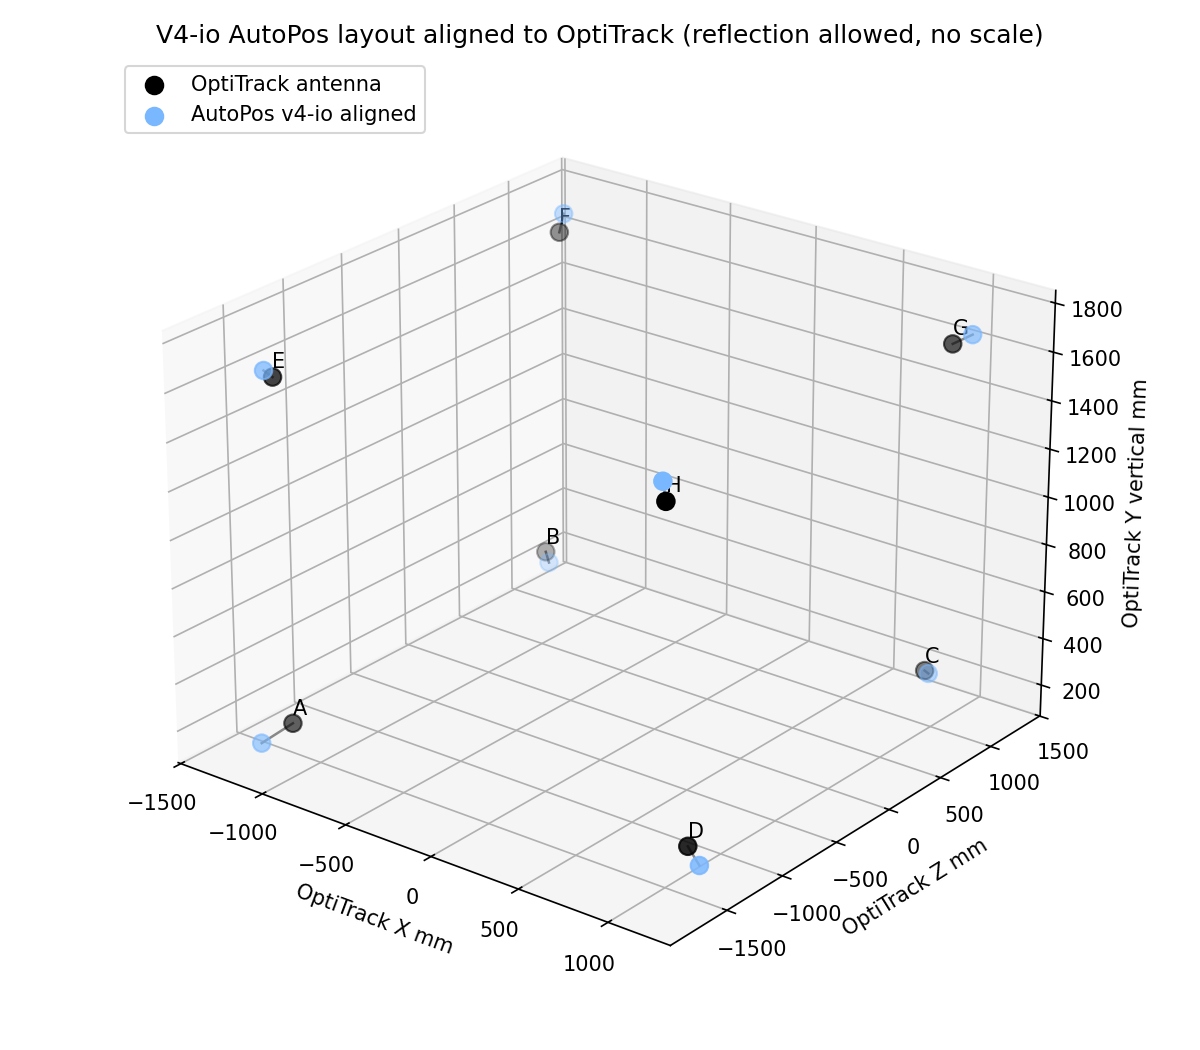
\includegraphics[width=0.78\textwidth]{layout_opti_vs_autopos_3d.png}
\caption{Vicon Motion Capture System anchor layout 与 AutoPos \case{v4-io} layout 的三维比较。该图用于说明 AutoPos 不是完全随机地恢复锚点结构，而是在真实坐标系下有可解释的刚体误差和尺度偏差。}
\end{figure}

AutoPos \case{v4-io} 布局相对于 Vicon Motion Capture System 锚点的刚体 SE(3) RMSE 为 $105.4\mm$。如果允许 Sim(3) 尺度校正，残差降到 $67.1\mm$，对应约 $-4.17\%$ 的 scale bias。这说明布局误差包含两层：一层是整体尺度或延迟造成的系统性偏差，另一层才是锚点相对形状的残差。

这个结果的写法要谨慎。不能说 AutoPos ``完全等于'' Vicon Motion Capture System，也不能说它失败。更准确的表述是：AutoPos 在真实测距条件下恢复出了可用拓扑和近似几何，但 UWB 测距延迟和布局尺度互相耦合，使得绝对尺度仍需要 calibration 或更强约束。

\section{Delay-layout coupling：本报告最重要的机制证据}

\begin{figure}[H]
\centering
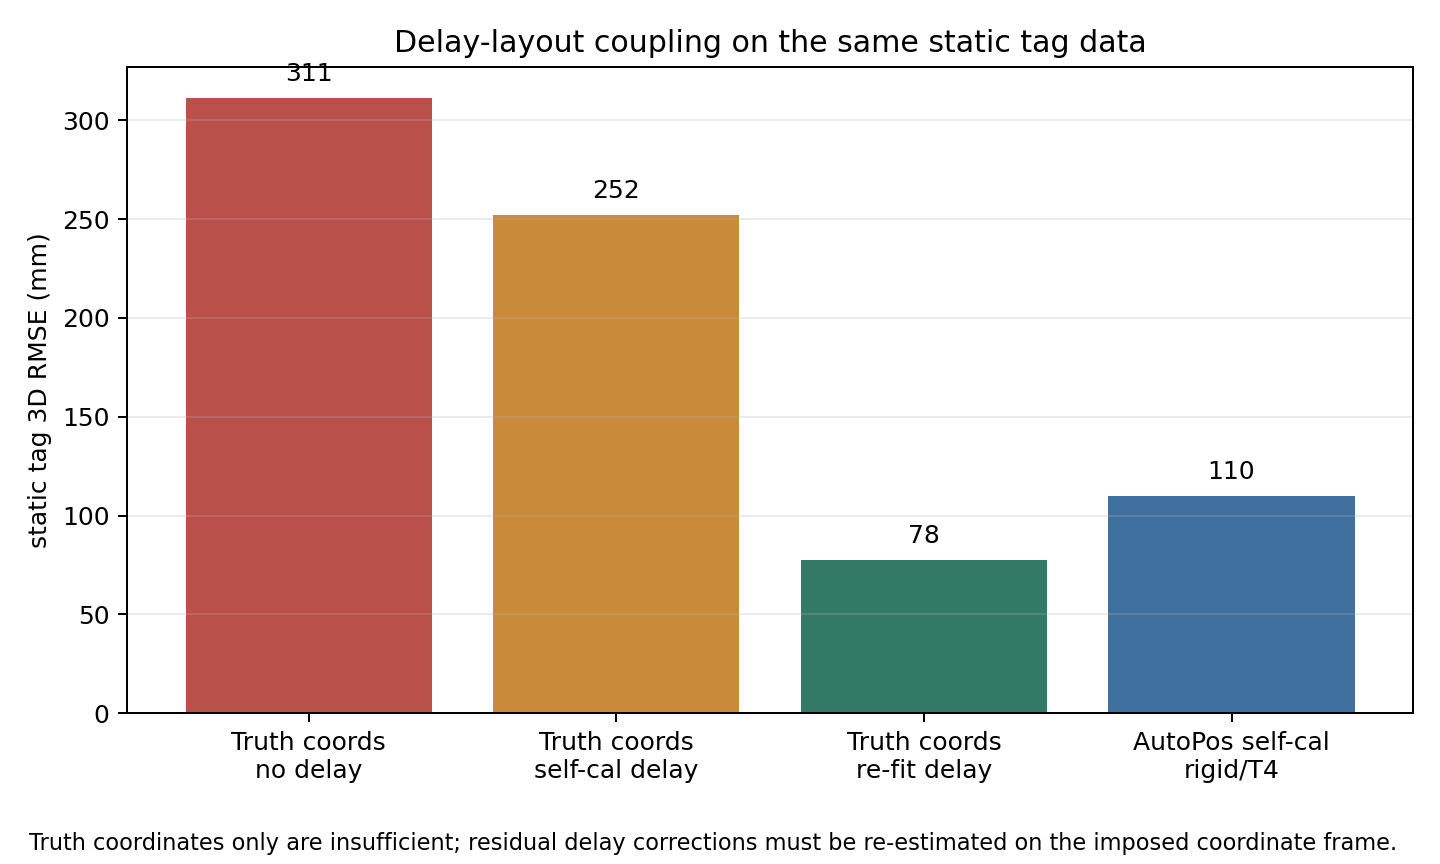
\includegraphics[width=0.78\textwidth]{delay_layout_coupling.png}
\caption{锚点布局与 delay calibration 的耦合关系。仅替换 Vicon Motion Capture System 锚点而不重新估计 delay，并不会自动得到好结果。}
\end{figure}

\begin{table}[H]
\centering
\caption{Delay-layout coupling 对照。所有 RMSE 单位为 mm。}
\begin{tabular}{@{}l r l@{}}
\toprule
配置 & RMSE & 说明 \\
\midrule
Vicon anchors，无 delay correction & 311.3 & 真值锚点不等于好定位，delay 错误会主导误差。 \\
Vicon anchors，移植 AutoPos delay & 252.2 & delay 不能直接从一个 layout 搬到另一个 layout。 \\
Vicon anchors，重新估计 delay & 77.7 & 锚点真值与匹配 delay 一起使用时，静态定位显著改善。 \\
AutoPos \case{v4-io}，co-fitted delay & 108.9 & 自定位布局和 delay 一起拟合后达到部署级可用精度。 \\
\bottomrule
\end{tabular}
\end{table}

这组对照应该作为报告的机制核心。它说明真实系统中有一个三角关系：锚点布局、测距延迟、tag solver 是一起工作的。Vicon Motion Capture System 锚点虽然几何更准，但如果 delay model 没有跟着重新估计，结果反而可能很差。因此主报告不能只展示 ``AutoPos vs Vicon Motion Capture System layout''，还必须解释 delay-layout coupling。

\section{静态 tag 定位结果}

\begin{figure}[H]
\centering
\begin{subfigure}{0.49\textwidth}
\centering
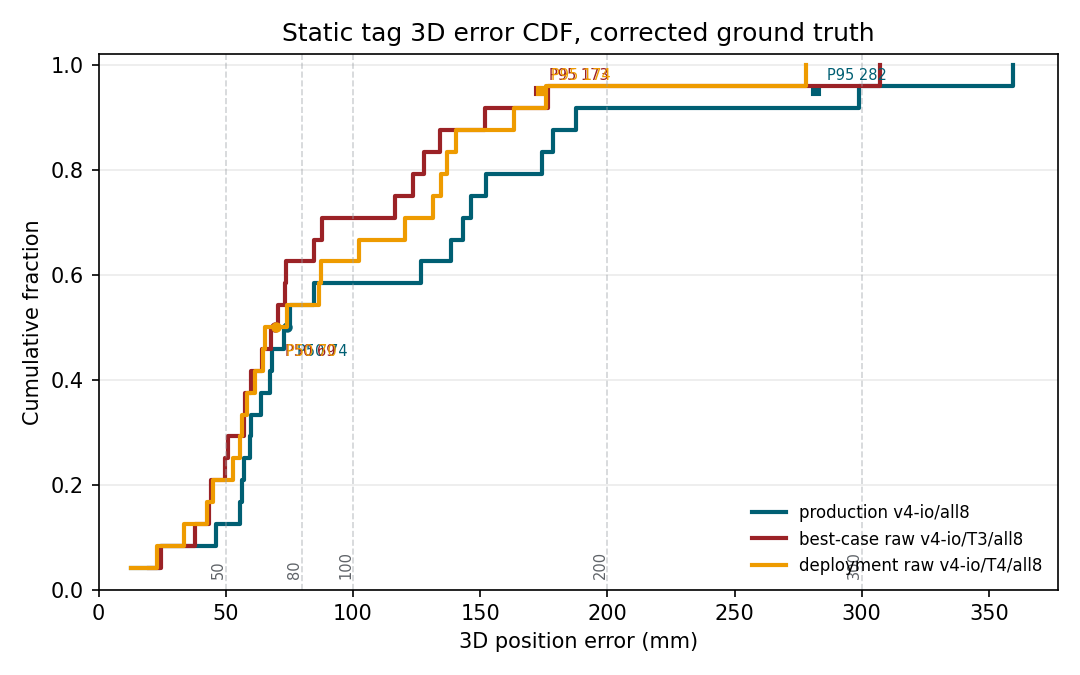
\includegraphics[width=\textwidth]{tag_error_cdf.png}
\caption{整体误差 CDF}
\end{subfigure}
\begin{subfigure}{0.49\textwidth}
\centering
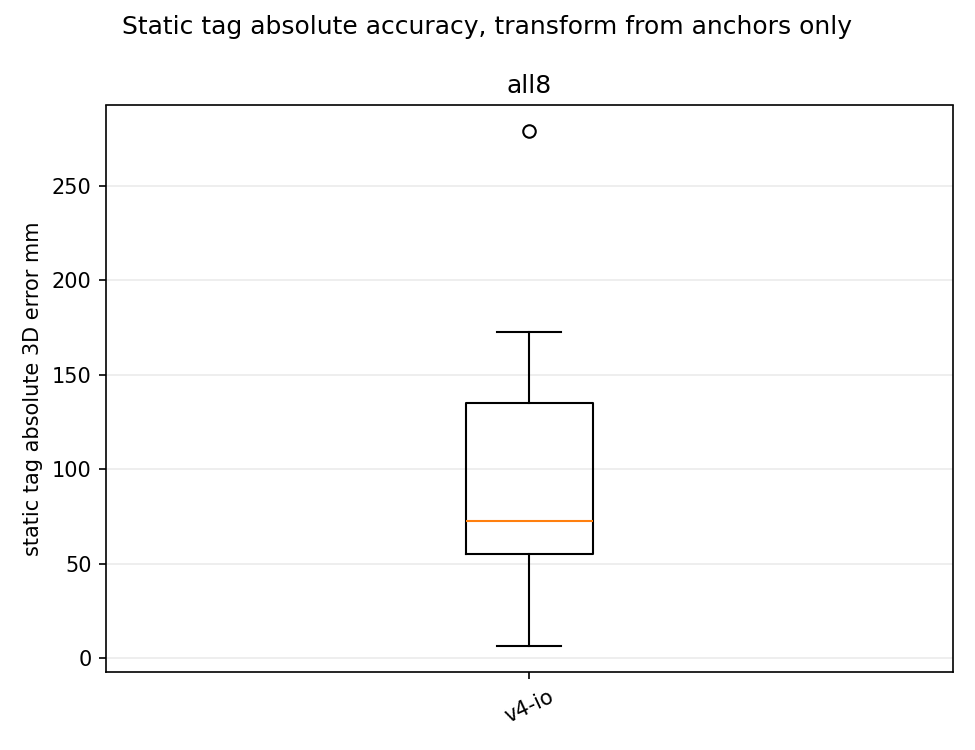
\includegraphics[width=\textwidth]{static_tag_error_by_position.png}
\caption{AutoPos Solver 与 UWB-Tag solver 组合按位置分解}
\end{subfigure}
\caption{静态 UWB-Tag 定位的主结果视图。建议正文优先报告 \case{v4-io/T4} 这个 AutoPos Solver 与 UWB-Tag solver 组合，而不是把估计器消融的更低 median 当作主结果。}
\end{figure}

\begin{figure}[H]
\centering
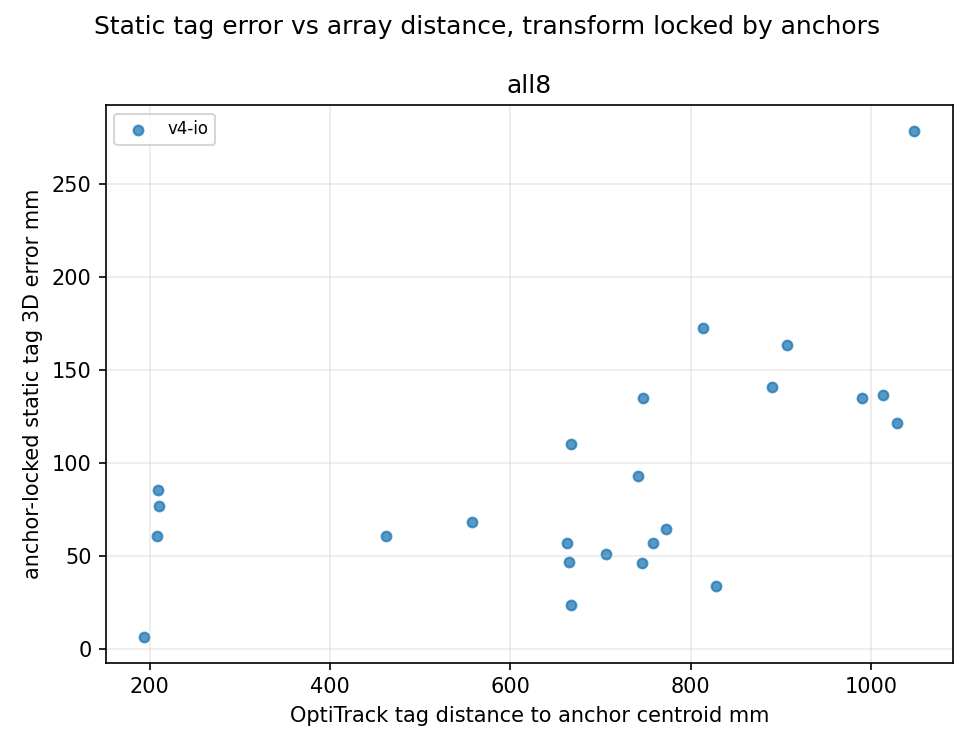
\includegraphics[width=0.72\textwidth]{static_tag_error_vs_distance.png}
\caption{AutoPos Solver 与 UWB-Tag solver 组合下误差与 tag-anchor 距离关系。该图适合用于讨论几何条件、距离相关 bias 和边缘点误差。}
\end{figure}

静态定位的推荐 headline 是：
\[
\case{v4-io/T4}: \quad \mathrm{median}=72.7\mm,\quad \mathrm{P95}=171.5\mm,\quad \mathrm{RMSE}=109.8\mm.
\]
这个数字代表 AutoPos Solver 与 UWB-Tag solver 组合 \case{v4-io/T4} 的主结果，应作为摘要、结论和表格中的主结果。之前分析中出现的 $69.7\mm$ median、$173.9\mm$ P95 是 median-estimator 消融结果，不能写成主结果。正确写法是：估计器选择会轻微改变 median，但系统级结果仍应以 $72.7/171.5/109.8\mm$ 为准。

\subsection{静态滤波的意义}

\begin{figure}[H]
\centering
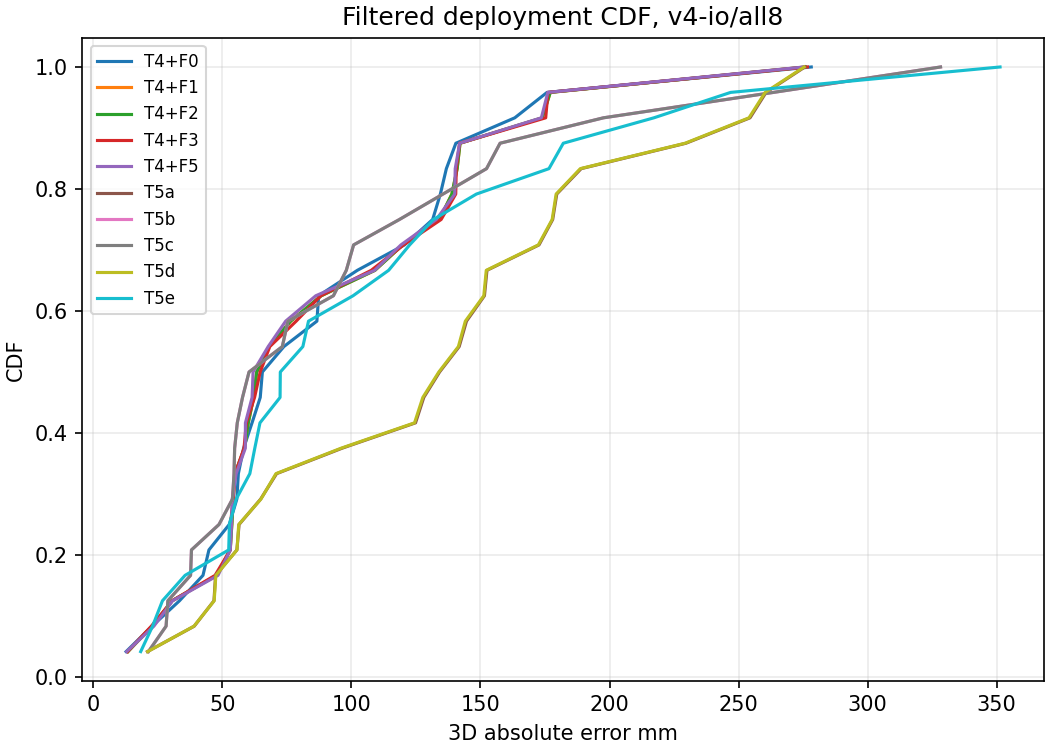
\includegraphics[width=0.75\textwidth]{filtered_static_cdf_v4io_all8.png}
\caption{静态滤波对 repeatability 的影响。F5 可以显著降低重复测量 spread，但不能消除系统性偏差。}
\end{figure}

静态 lock/filter F5 将 repeatability spread 从 $67.4\mm$ 降到 $18.7\mm$。这说明滤波非常适合提高静态读数稳定性，例如展示界面、长期占位、慢速更新。但这个结果不应被解释为锚点布局或 delay calibration 被修正；它主要降低随机波动，对固定 bias 的影响有限。

\section{动态 RotoArm UWB-Tag：为什么比静态更难}

\begin{figure}[H]
\centering
\begin{subfigure}{0.49\textwidth}
\centering
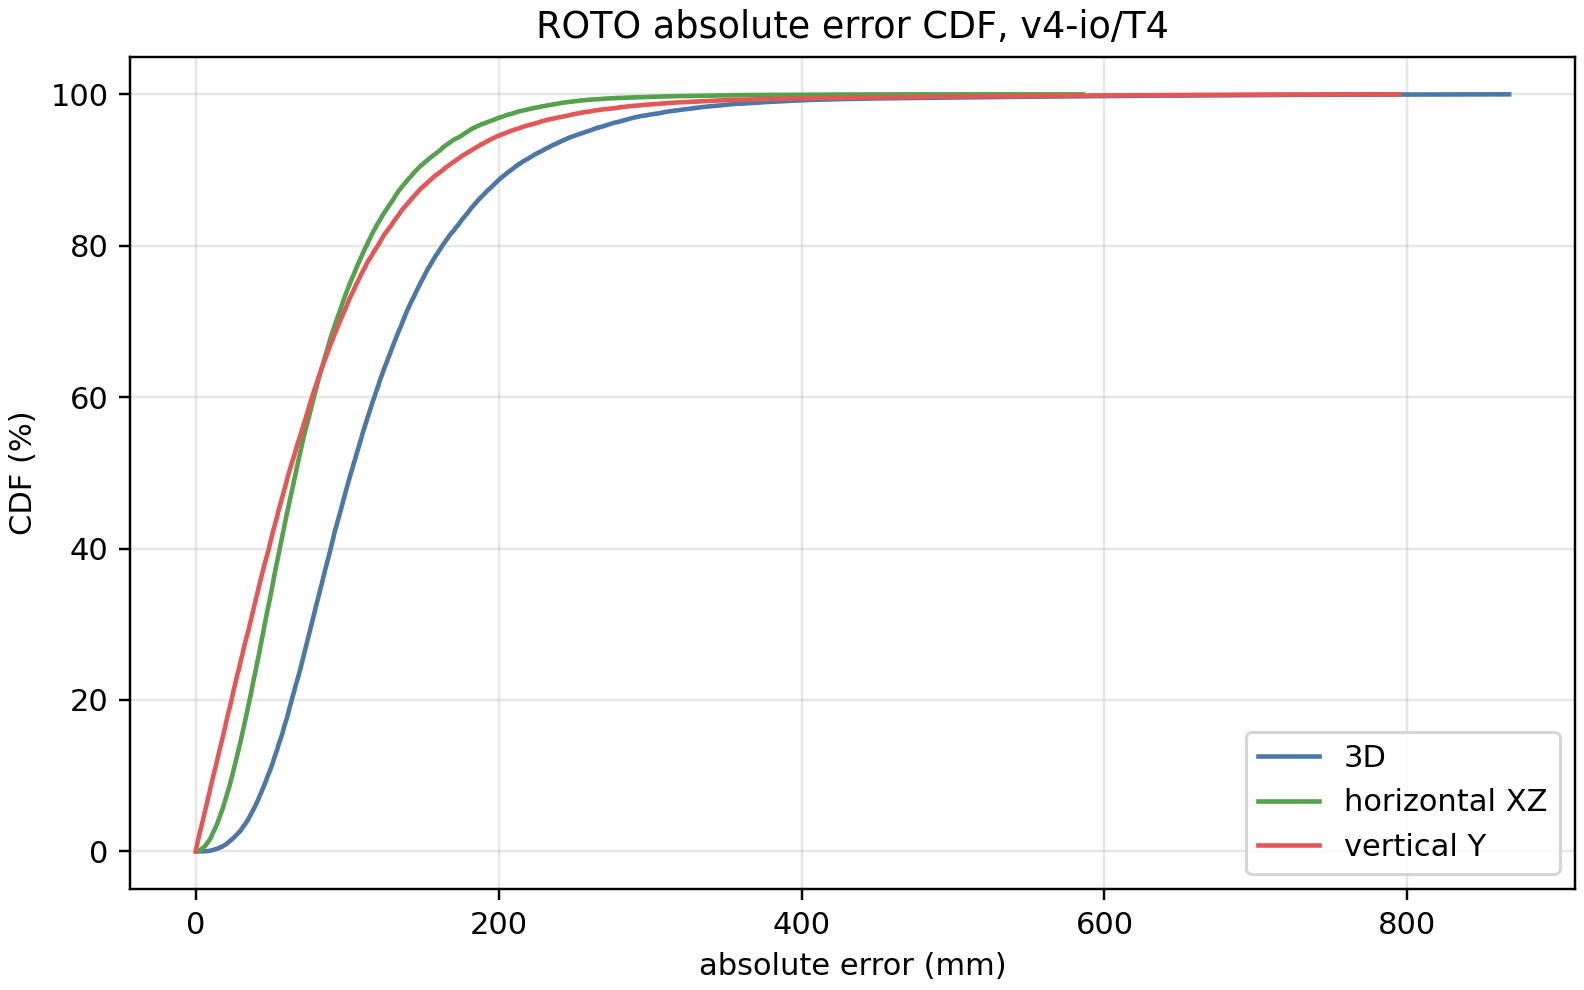
\includegraphics[width=\textwidth]{roto_abs_cdf_v4io_T4.png}
\caption{RotoArm UWB-Tag 绝对误差 CDF}
\end{subfigure}
\begin{subfigure}{0.49\textwidth}
\centering
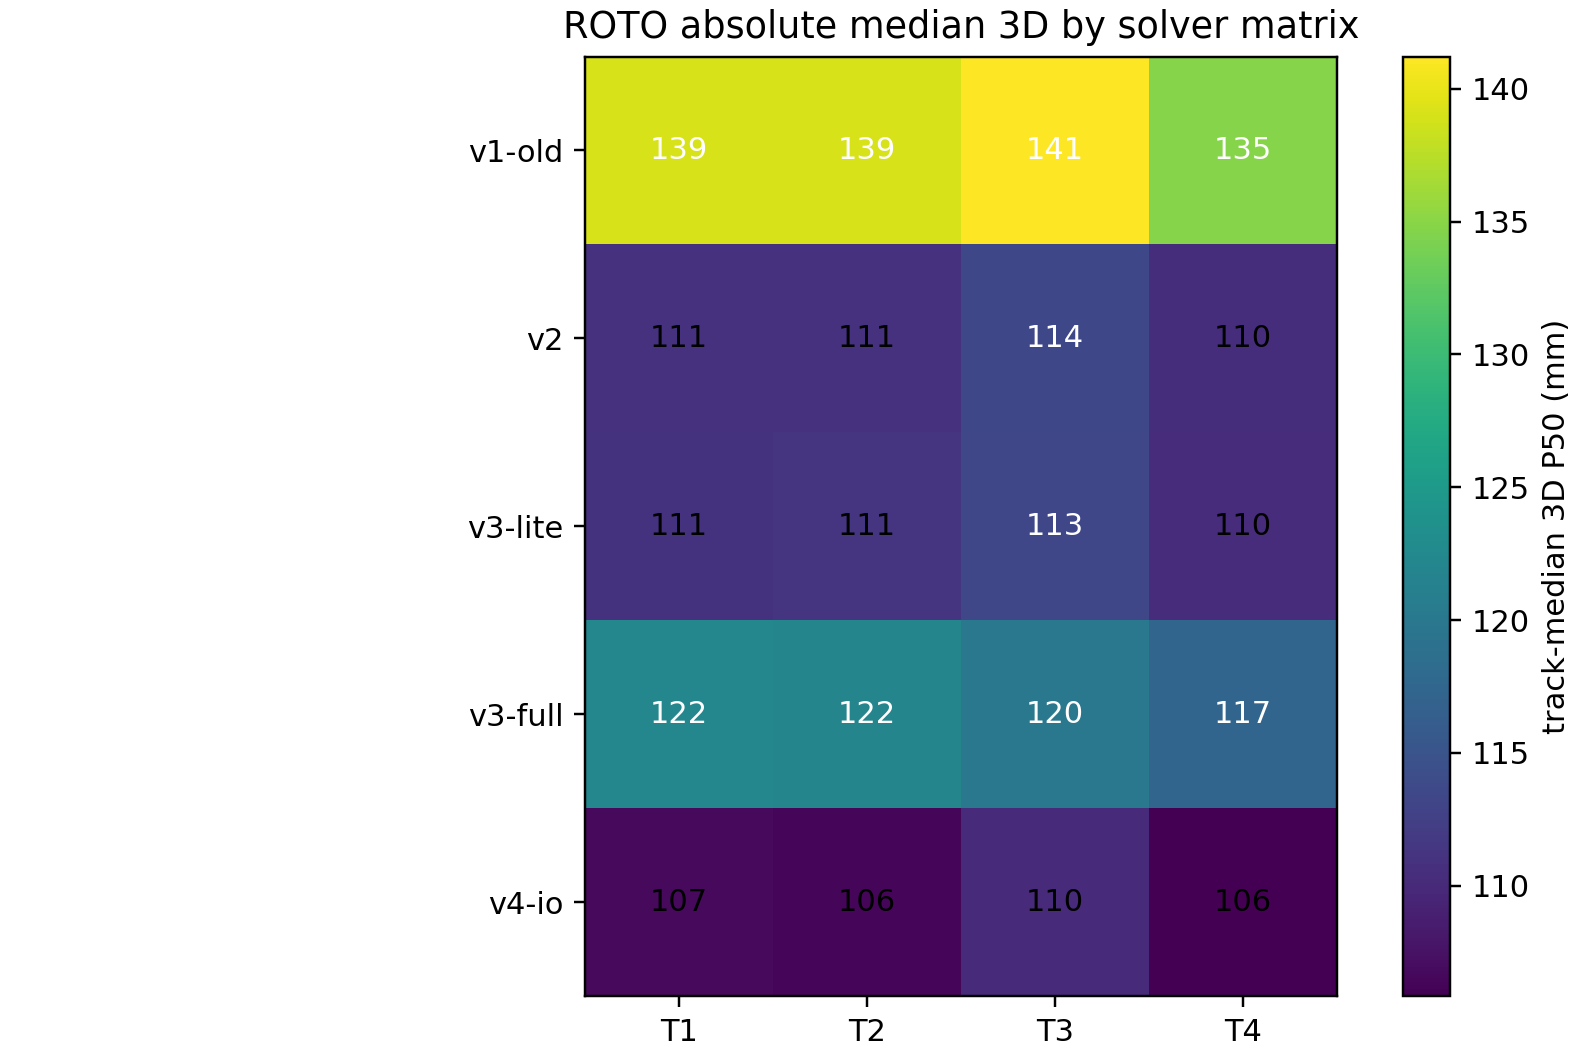
\includegraphics[width=\textwidth]{roto_solver_matrix_median3d.png}
\caption{RotoArm UWB-Tag solver 矩阵}
\end{subfigure}
\caption{动态 RotoArm UWB-Tag 结果。RotoArm UWB-Tag 误差高于静态结果，说明动态轨迹中存在额外误差源。}
\end{figure}

\begin{figure}[H]
\centering
\begin{subfigure}{0.49\textwidth}
\centering
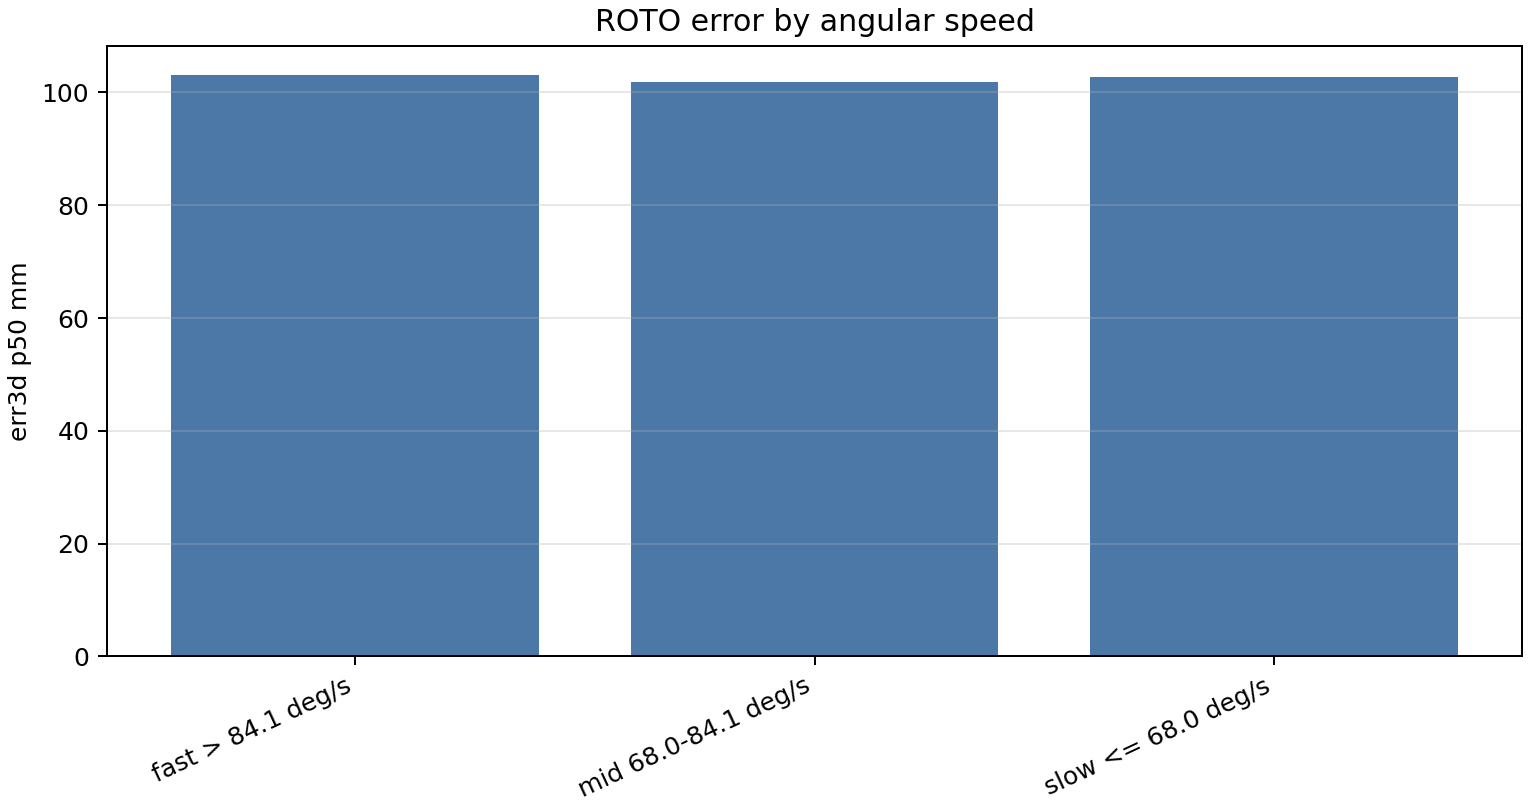
\includegraphics[width=\textwidth]{roto_error_by_angular_speed.png}
\caption{按角速度分解}
\end{subfigure}
\begin{subfigure}{0.49\textwidth}
\centering
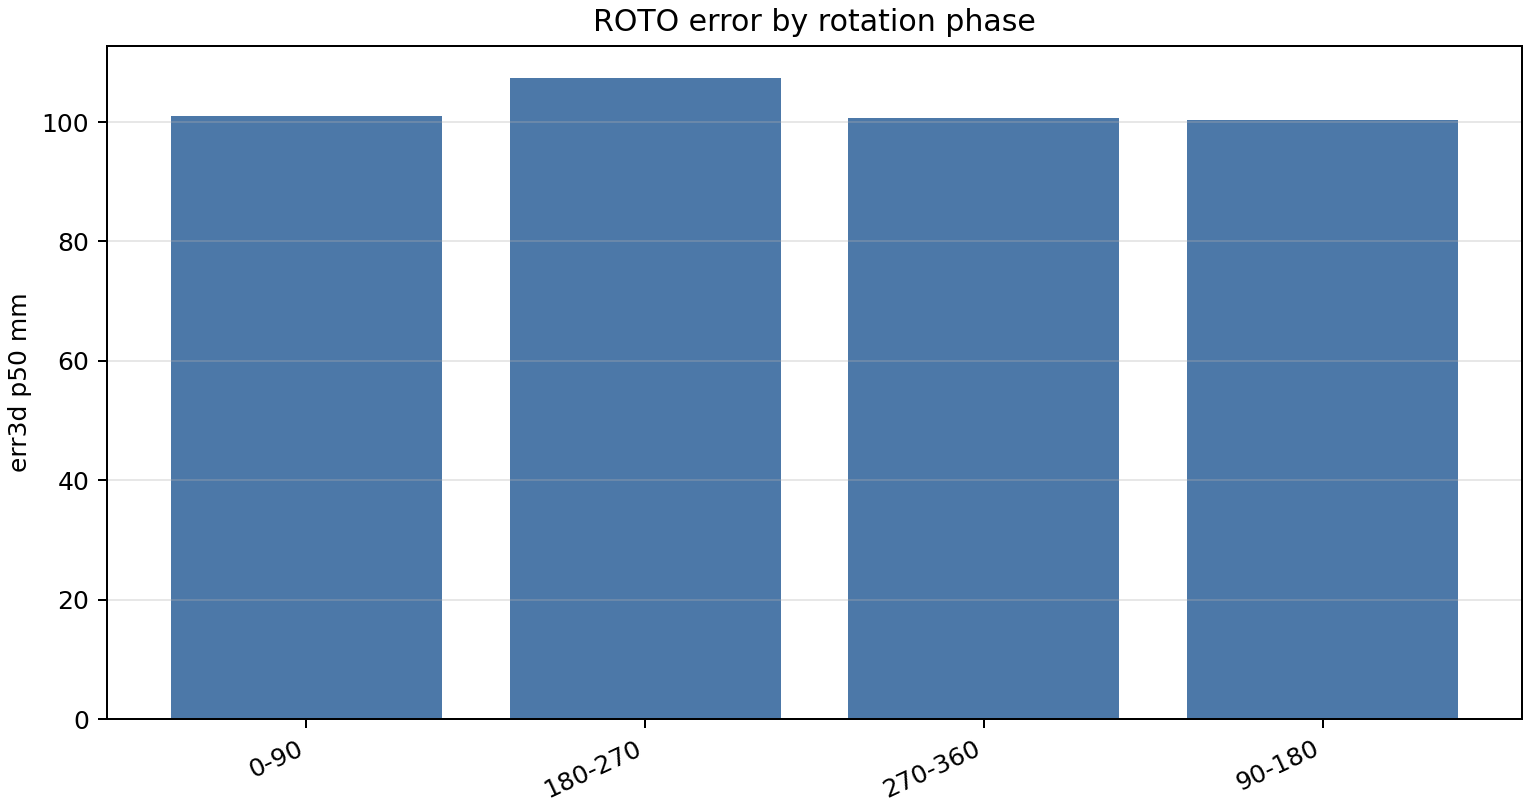
\includegraphics[width=\textwidth]{roto_error_by_phase.png}
\caption{按运动 phase 分解}
\end{subfigure}
\caption{RotoArm UWB-Tag 动态诊断图。它们适合支持 ``动态误差不是简单静态 bias'' 这一判断。}
\end{figure}

\case{v4-io/T4} 的 RotoArm UWB-Tag 原始绝对误差为 $105.8\mm$ median、$231.8\mm$ P95、$141.3\mm$ sample RMSE。即使使用 Vicon anchors 并重新估计 delay，RotoArm UWB-Tag 仍约为 $105.6\mm$ median、$200.4\mm$ P95。这是非常关键的负结果：动态 RotoArm UWB-Tag 的主要问题不能只靠换成 Vicon Motion Capture System anchor layout 解决。

时间相关检查同样支持这个判断。时钟 skew 对 pooled P50 的影响约 $0.11\mm$，而 $0.8\mathrm{ms}$ protocol window 按当前运动速度只对应约 $0.5$--$0.7\mm$ 位移。因此，RotoArm UWB-Tag 的百毫米级误差不太可能由简单时间窗解释。更合理的解释是动态条件下的 range bias、人体遮挡、天线朝向、multipath/NLOS 和 solver 动态假设共同作用。

RotoArm UWB-Tag 的 F4/F5 滤波结果可以作为工程展示：F4 约 $86.3\mm$ median、$158.2\mm$ P95，F5 约 $83.3\mm$ median、$148.6\mm$ P95。但正文中要强调它们是 post-solve smoother，不是 calibration。它们能让轨迹更平滑，却不能证明原始测距物理误差已经被消除。

\section{Monte Carlo keep-k：锚点缺失稳健性}

\begin{figure}[H]
\centering
\begin{subfigure}{0.49\textwidth}
\centering
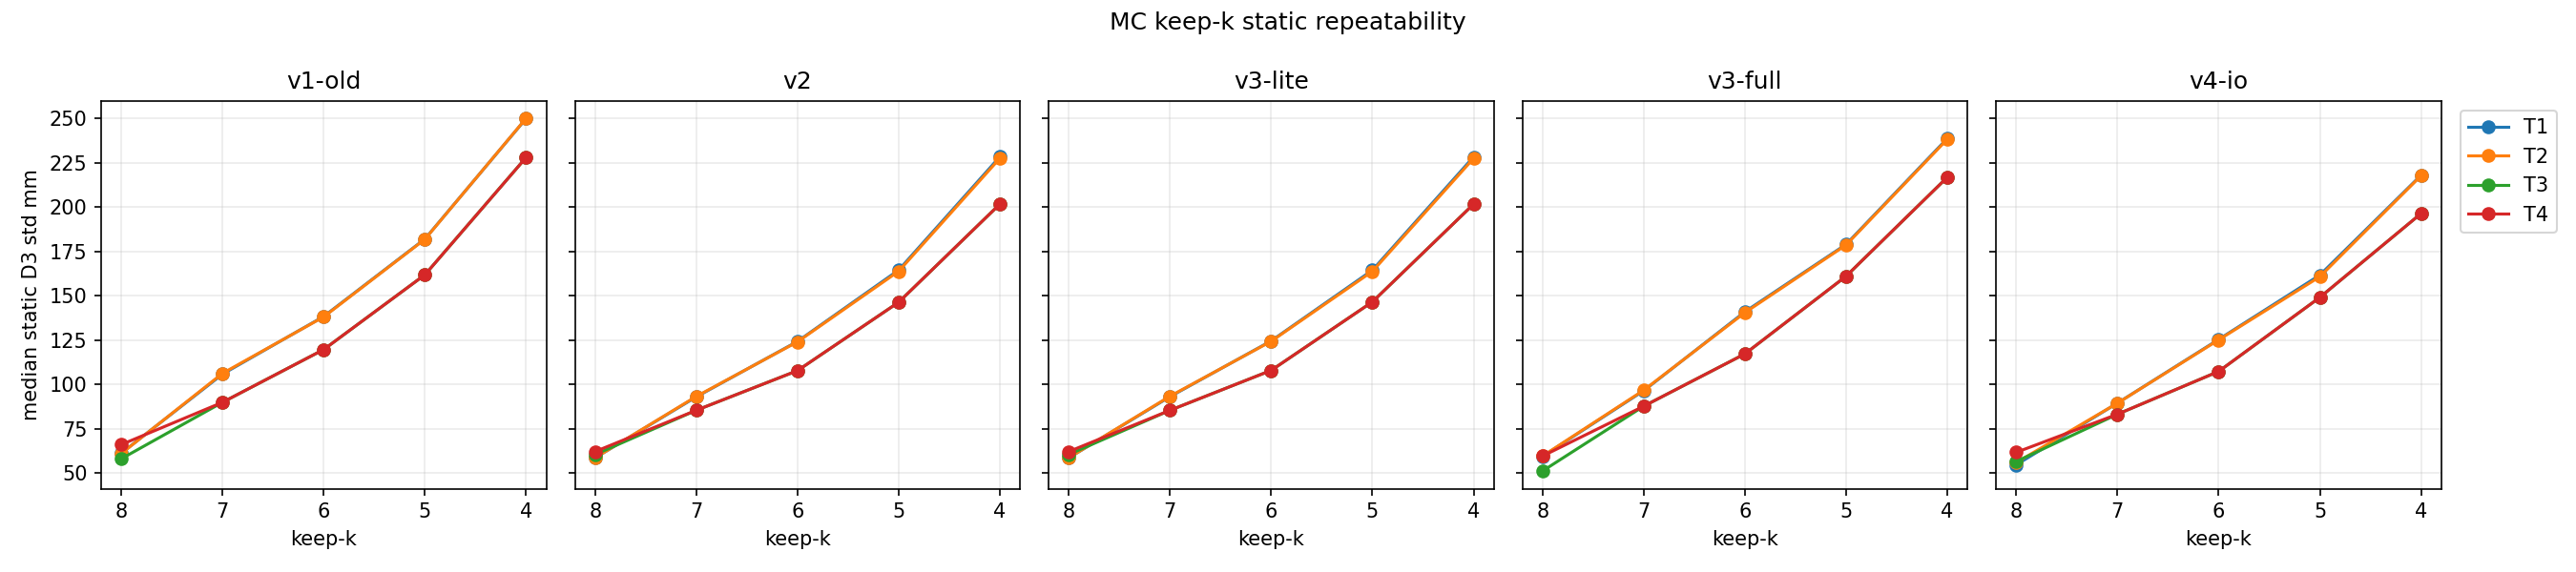
\includegraphics[width=\textwidth]{mc_keepk_static_curves.png}
\caption{静态 keep-k}
\end{subfigure}
\begin{subfigure}{0.49\textwidth}
\centering
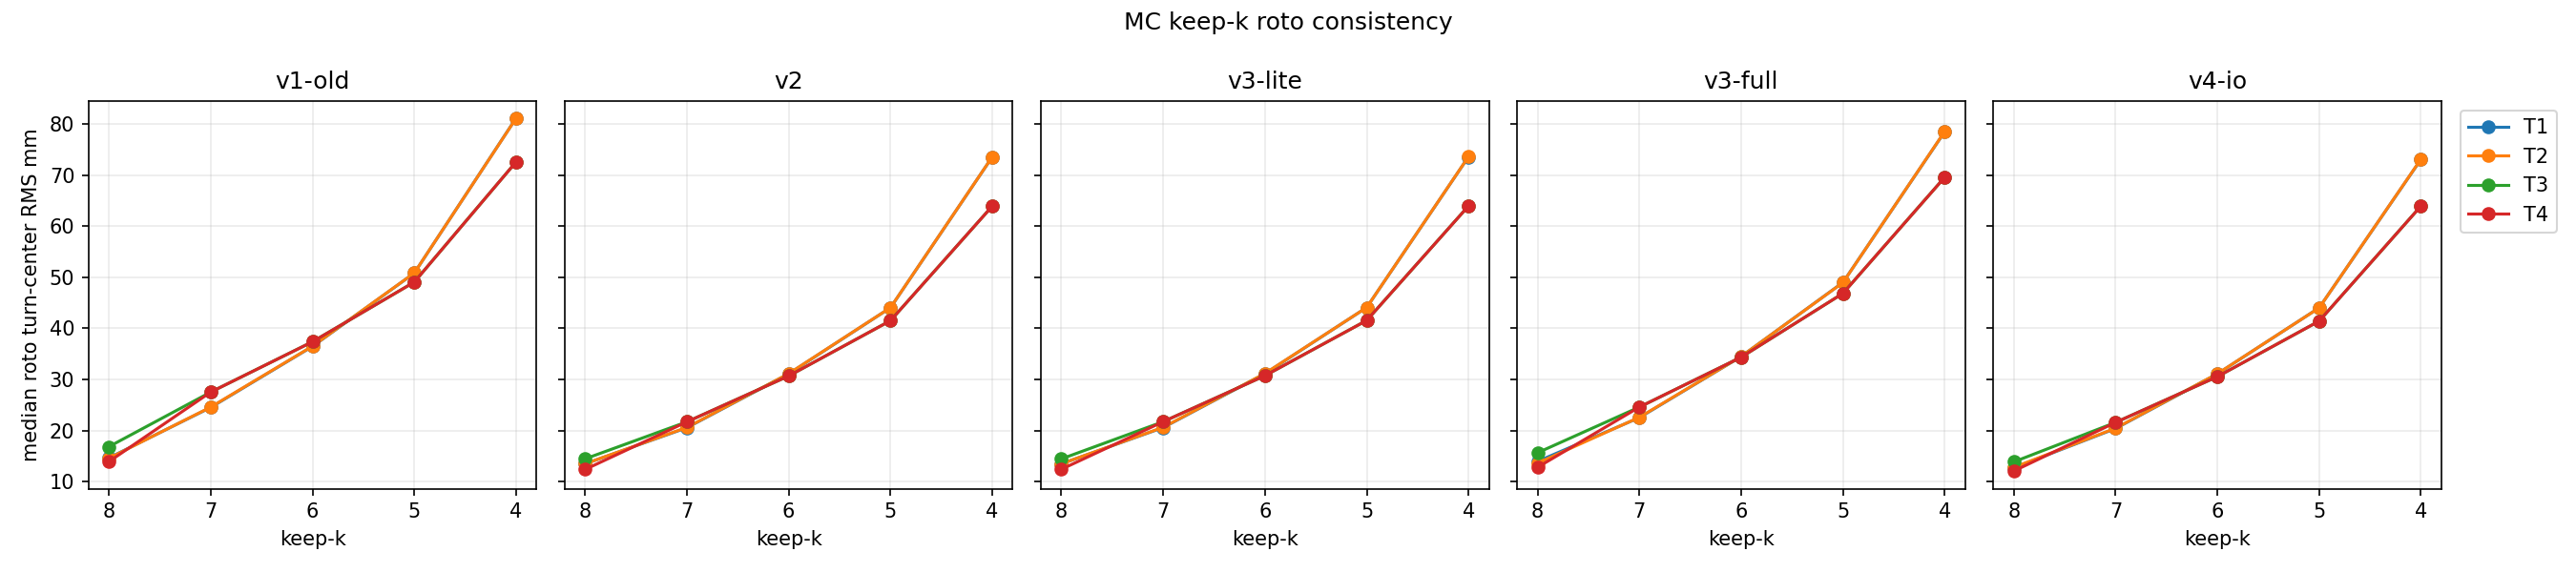
\includegraphics[width=\textwidth]{mc_keepk_roto_curves.png}
\caption{RotoArm UWB-Tag keep-k}
\end{subfigure}
\caption{Monte Carlo anchor availability stress test。它应该作为 robustness 章节，而不是主精度 headline。}
\end{figure}

\begin{figure}[H]
\centering
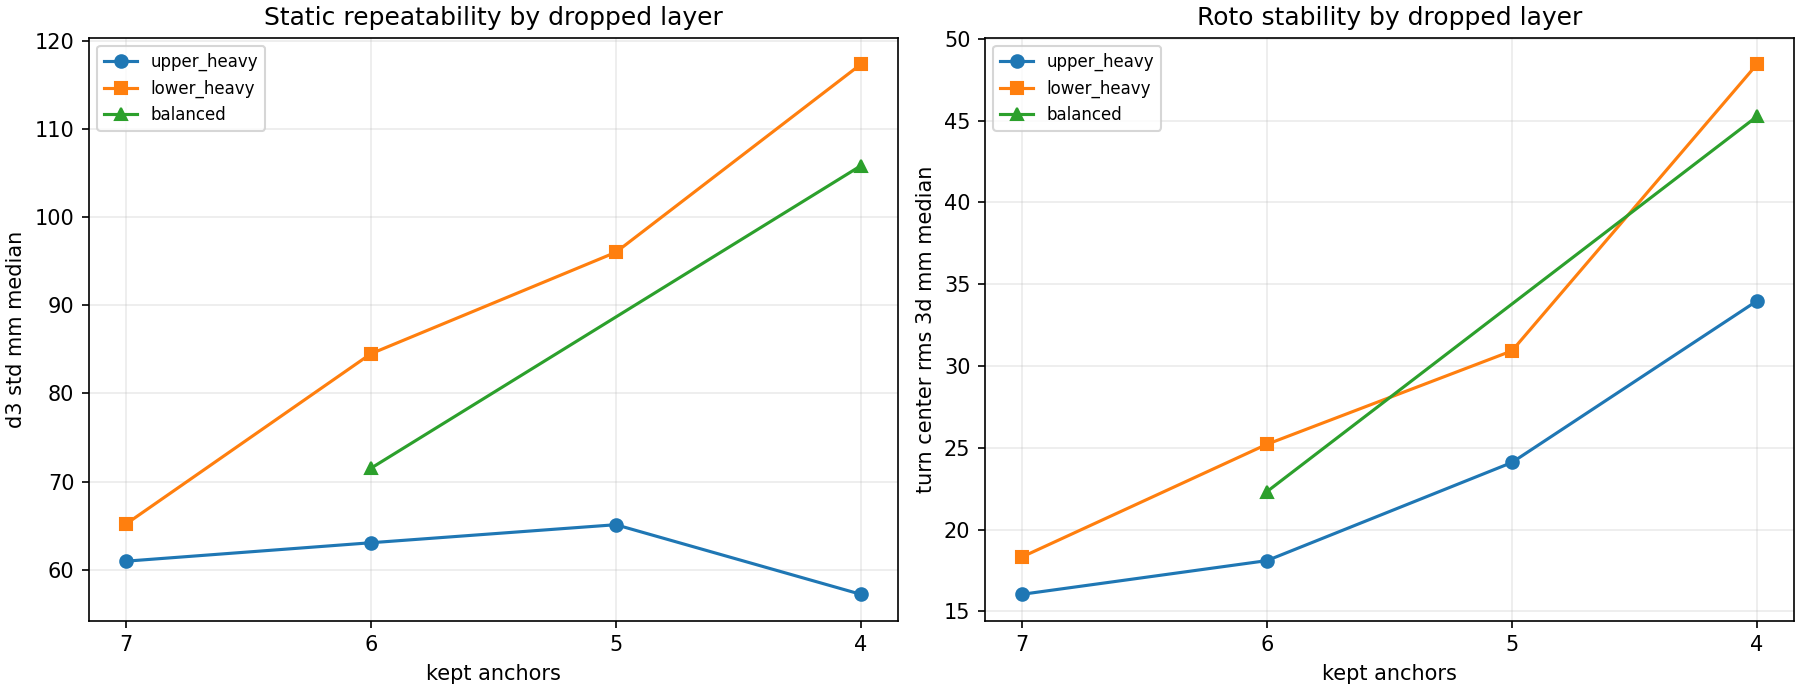
\includegraphics[width=0.72\textwidth]{stratified_keepk_upper_vs_lower.png}
\caption{按 upper/lower anchor drop 分层后的 keep-k 结果。低位锚点被移除时，静态结果明显更差。}
\end{figure}

Monte Carlo keep-k 结果说明锚点数量和空间分布对系统稳定性很重要。对于 \case{v4-io/T4}，静态 repeatability $d_3$ std median 从 keep8 的 $61.7\mm$ 上升到 keep7 的 $83.2\mm$、keep6 的 $107.3\mm$、keep5 的 $149.1\mm$ 和 keep4 的 $196.4\mm$。RotoArm UWB-Tag turn-center RMS median 也从 keep8 的 $12.1\mm$ 上升到 keep4 的 $63.9\mm$。

分层结果更有解释力：静态 keep5 lower-heavy drop 为 $96.0\mm$，upper-heavy drop 为 $65.1\mm$；keep4 lower-heavy 为 $117.3\mm$，upper-heavy 为 $57.2\mm$。这说明不是 ``少几个 anchor'' 这么简单，而是哪些空间层的 anchor 被移除会改变可观测性。报告中建议把这部分写成部署建议：保持上下层 anchor 覆盖，避免只剩单一高度平面的几何。

\section{仿真与 NLOS：为什么可以写，但不要喧宾夺主}

\begin{figure}[H]
\centering
\begin{subfigure}{0.49\textwidth}
\centering
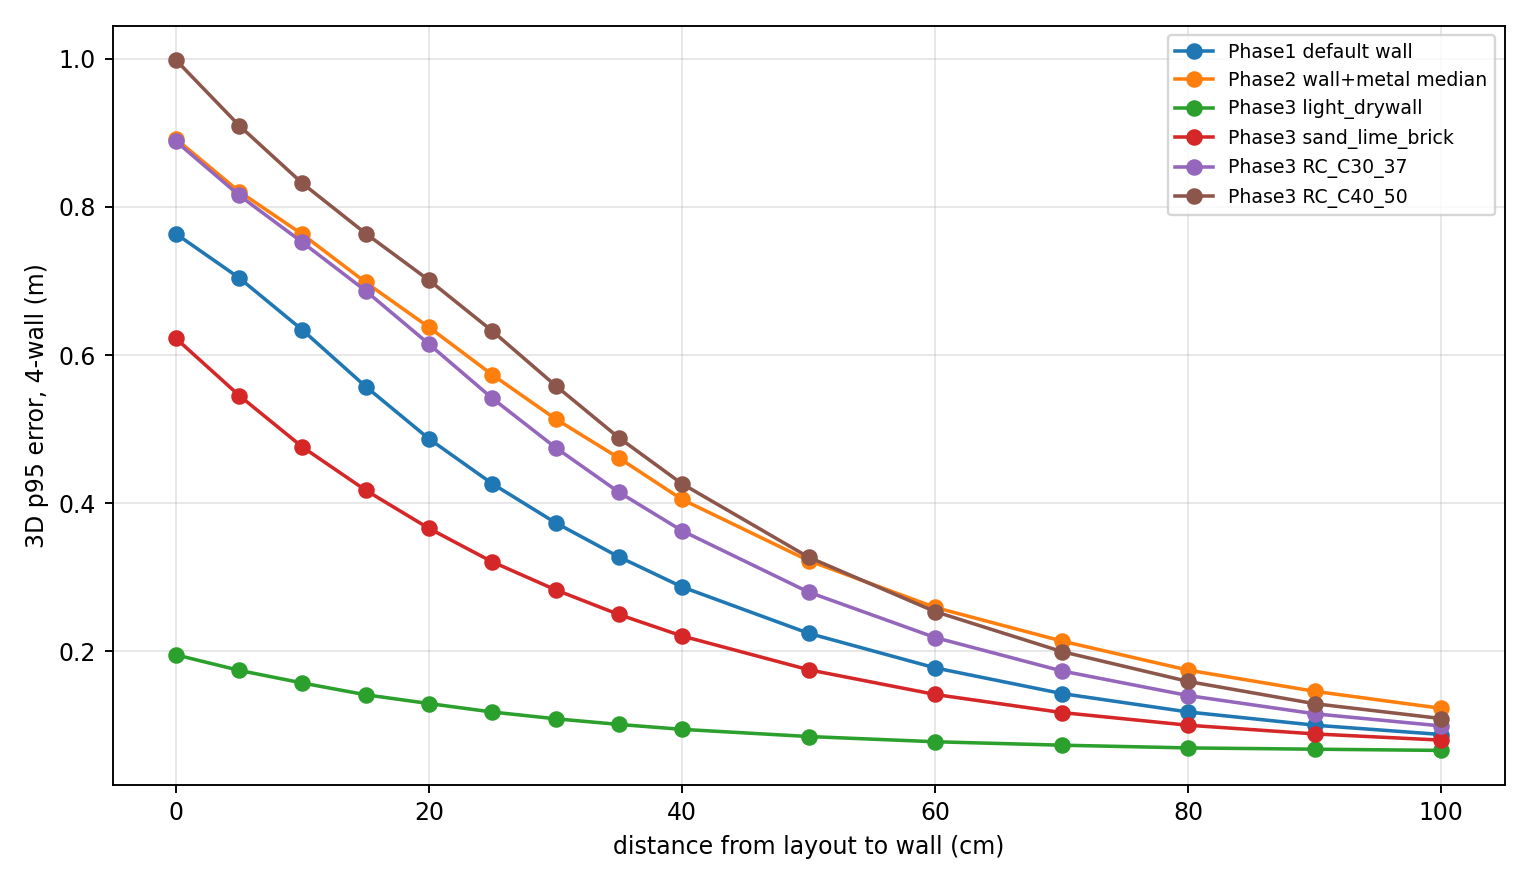
\includegraphics[width=\textwidth]{wall_nlos_p95_comparison.png}
\caption{墙体距离与 P95 误差}
\end{subfigure}
\begin{subfigure}{0.49\textwidth}
\centering
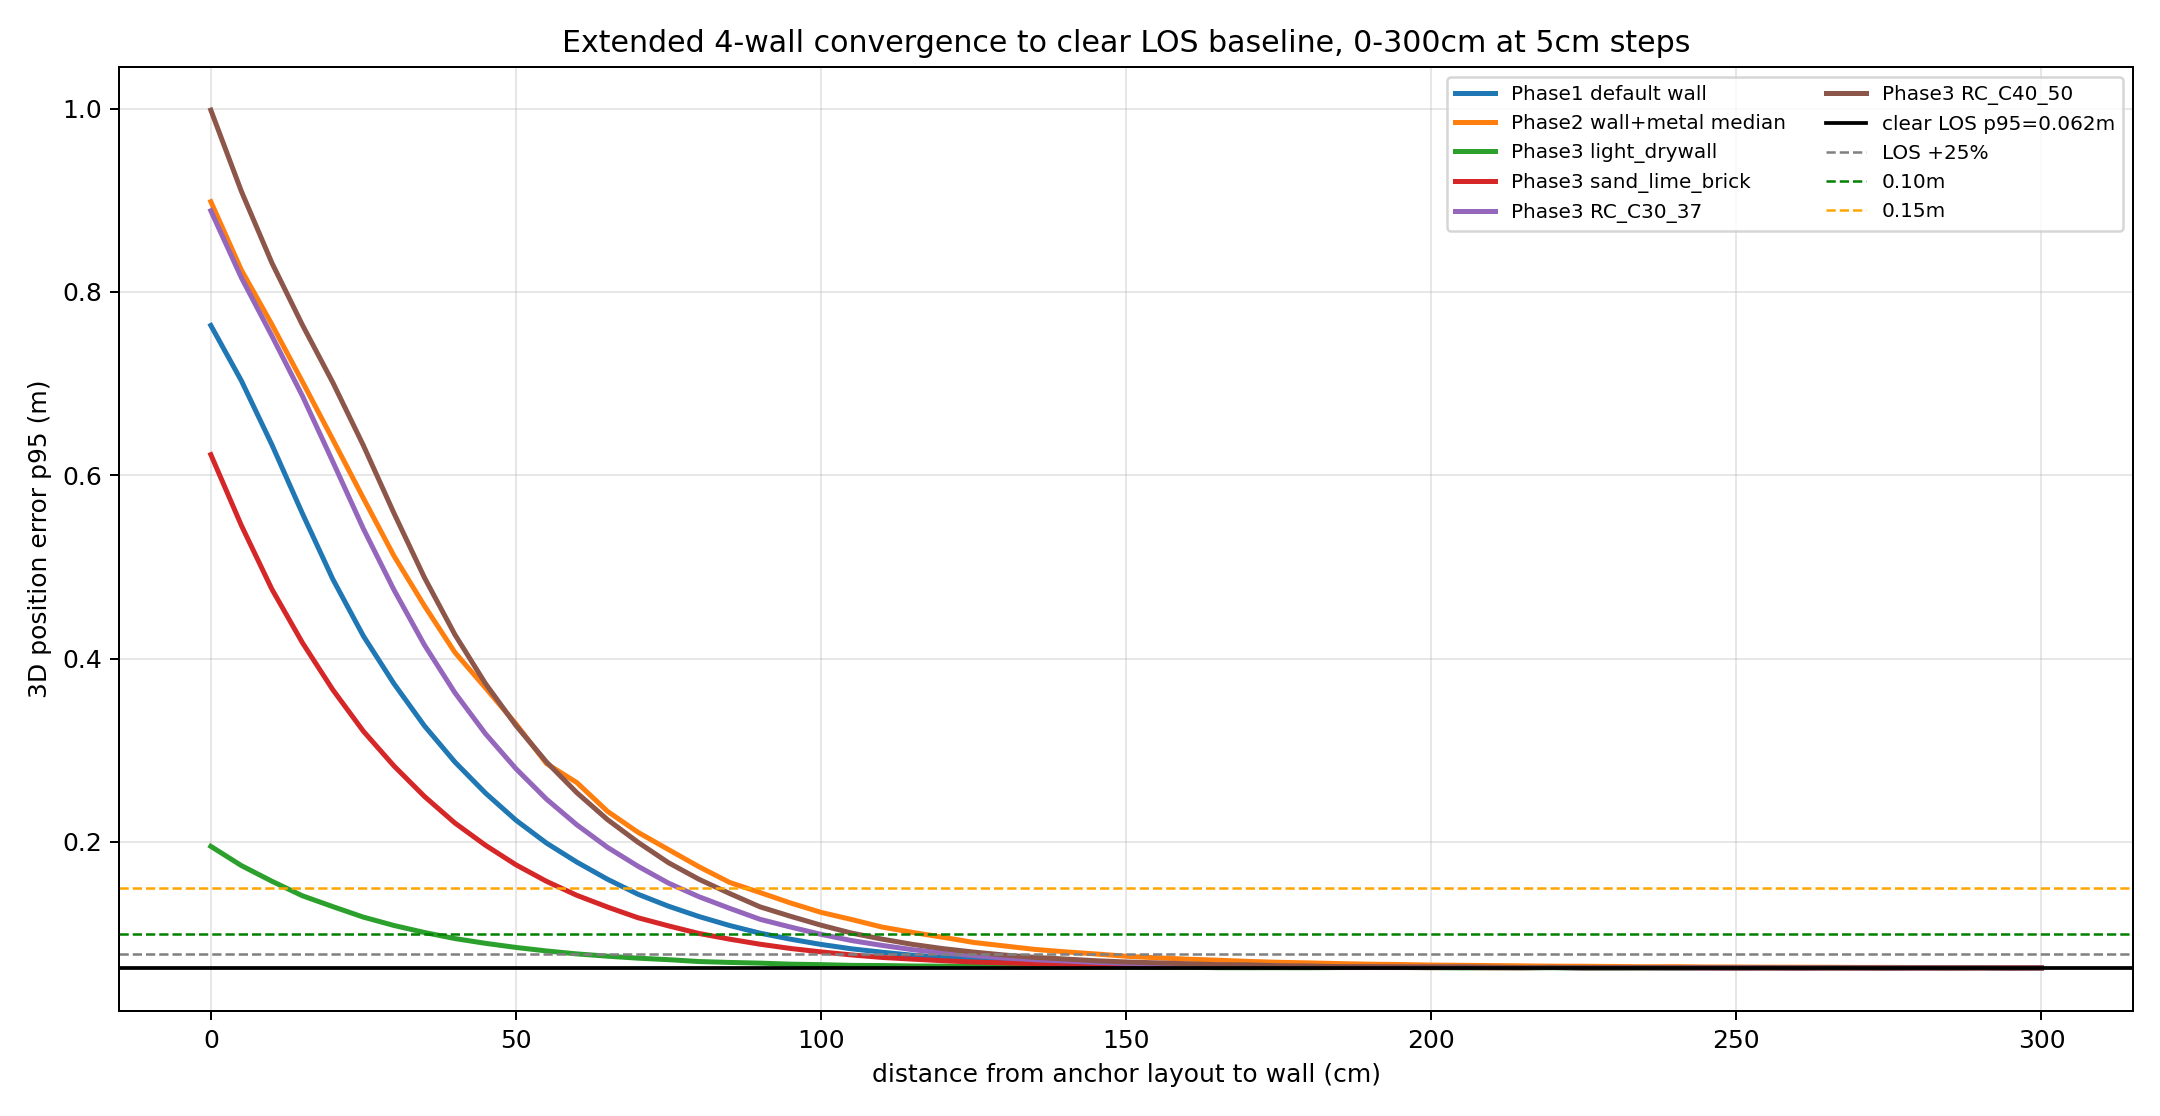
\includegraphics[width=\textwidth]{wall_nlos_convergence.png}
\caption{不同材料的收敛距离}
\end{subfigure}
\caption{AutoPos simulation 中的墙体 NLOS study。它可以解释 multipath/NLOS 风险，但不能替代真实实验评价。}
\end{figure}

\case{AutoPos_simulation} 是测量完成后的仿真研究，适合放在 discussion 或 supplementary。墙体 NLOS 仿真给出的趋势很清楚：clear LOS P95 约 $0.062\m$；4-wall default 在 0 cm、40 cm、100 cm 的 P95 分别约 $0.764\m$、$0.287\m$、$0.088\m$；4-wall+metal 分别约 $0.892\m$、$0.405\m$、$0.123\m$。extended convergence 结果显示 default wall 约 $115$ cm 才接近 LOS+25\%，wall+metal 约 $145$ cm。

这部分的写法应是：仿真支持一个物理解释，即靠近墙体、金属和遮挡环境时，range bias 可能显著放大定位尾部误差。因此它可以帮助解释 RotoArm UWB-Tag 和边缘位置的高 P95，也能自然引出 CIR/NLOS 检测的未来工作。但它不是同一套真实测量的独立验证，不能和 Vicon Motion Capture System-UWB 主结果混在同一个 headline 表里。

\section{Phase 4 UWB+IMU：L2/L16/L20 三类 IMU 对比}

\begin{figure}[H]
\centering
\begin{subfigure}{0.49\textwidth}
\centering
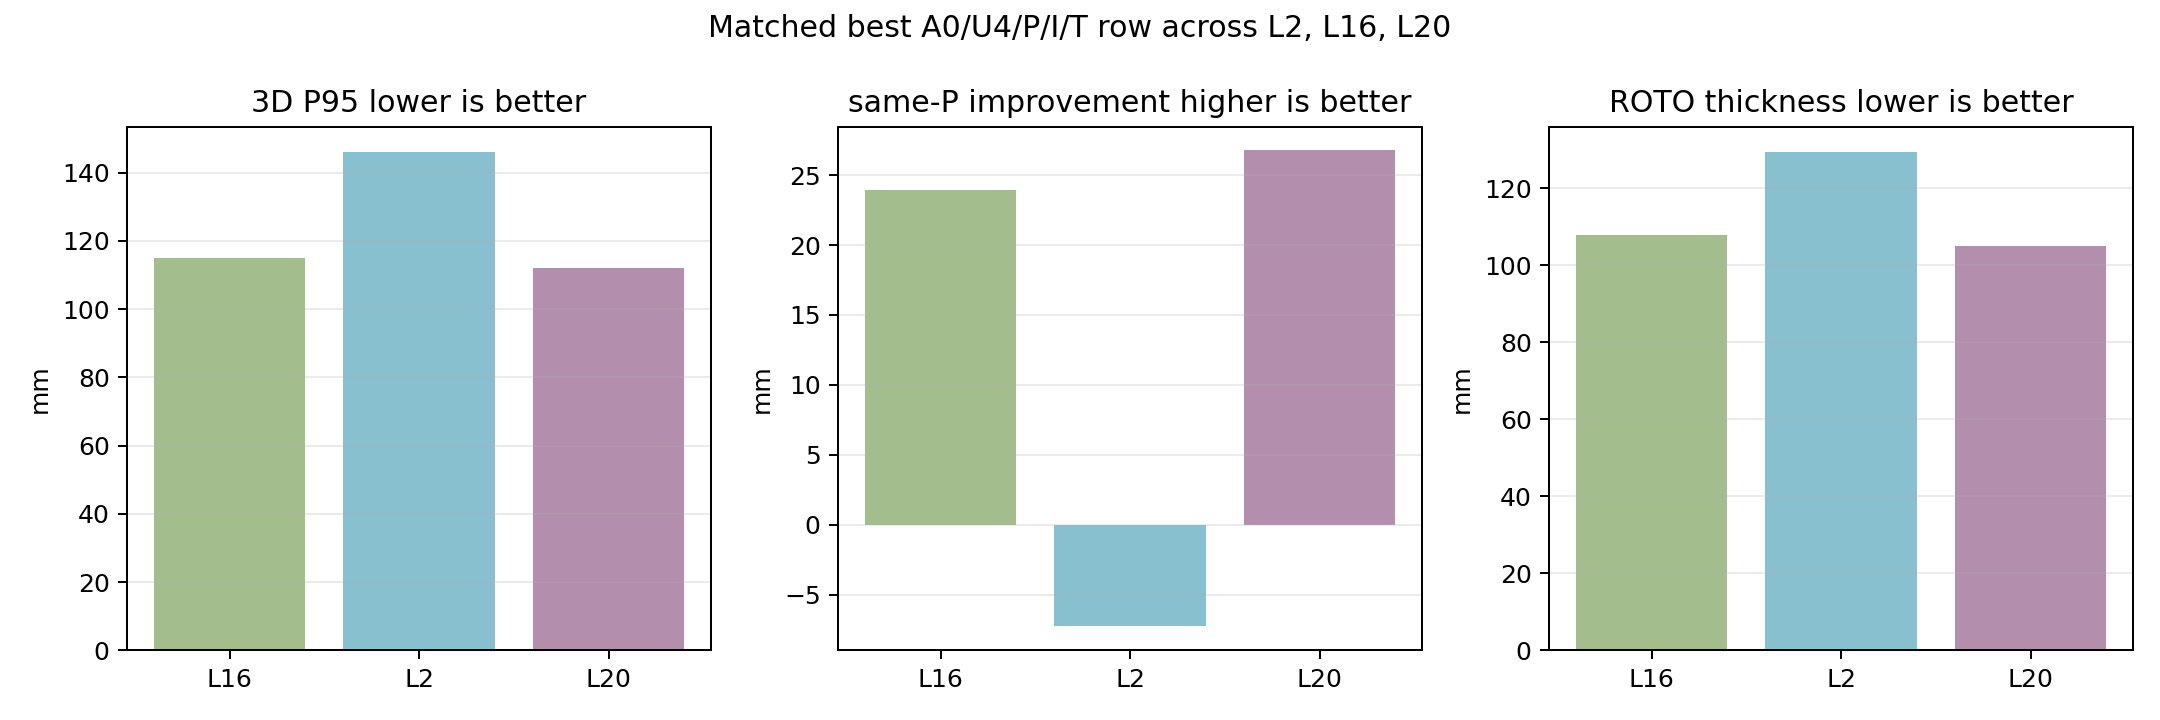
\includegraphics[width=\textwidth]{phase4_l2_l16_l20_sensor_comparison.png}
\caption{matched best combo 跨 sensor 对比}
\end{subfigure}
\begin{subfigure}{0.49\textwidth}
\centering
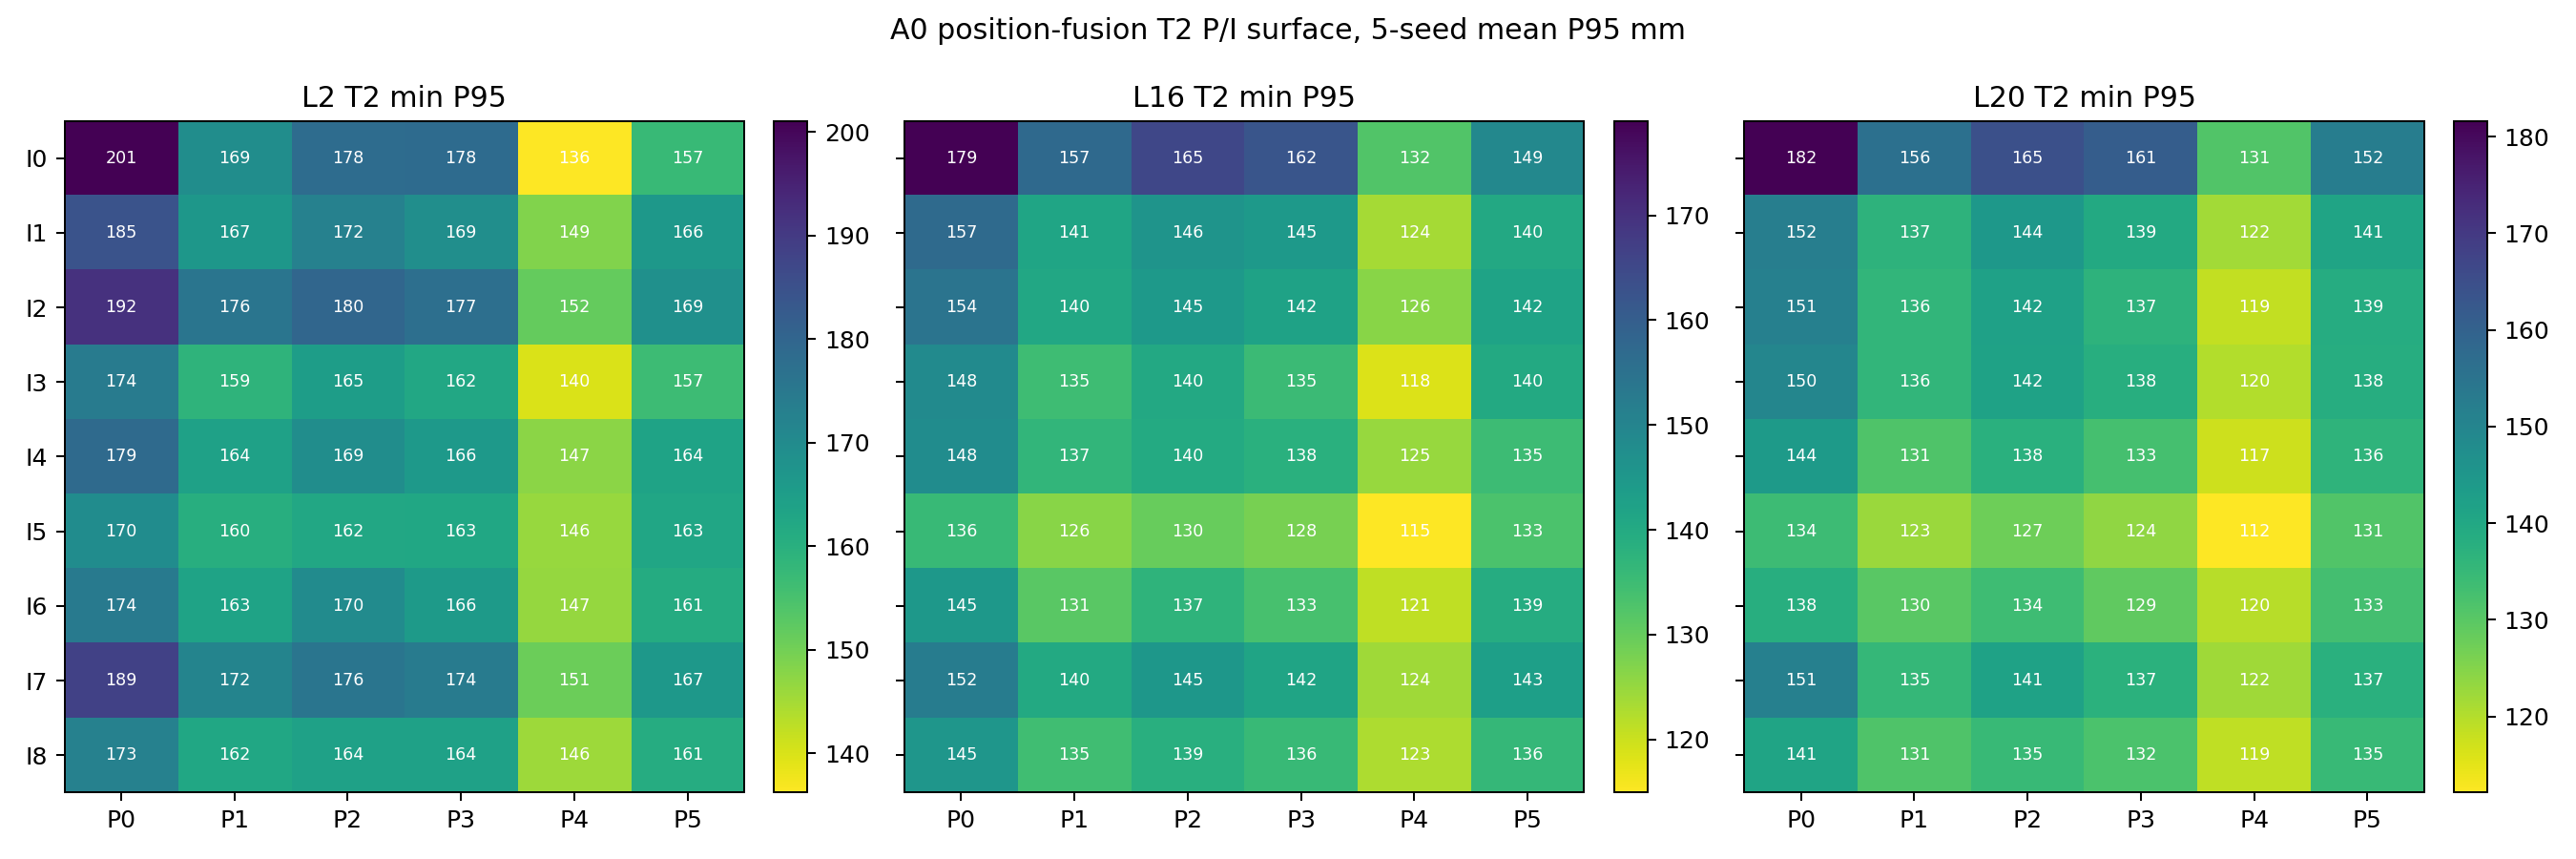
\includegraphics[width=\textwidth]{phase4_t2_pi_heatmap_by_sensor.png}
\caption{\case{T2} 分支下的 P/I heatmap}
\end{subfigure}
\caption{Phase 4 L2/L16/L20 TRUEFULL 5-seed Vicon-truth analysis。这里的 L 是 IMU sensor model，不是算法名称。}
\end{figure}

这里需要纠正一个容易写错的点：这一节不应该用早期 real 6-axis vertical slice 作为主结果。真正应该进入报告的是 2026年6月5日 生成的 Phase 4 L2/L16/L20 TRUEFULL 5-seed Vicon-truth analysis。该实验覆盖 L2、L16、L20 三类 IMU sensor model，每个 sensor 使用 S00--S04 五个 seed；每个 seed 有 1377 个 runnable rows、5292 个 declared rows，并用 RotoArm UWB-Tag Vicon trajectory 作为真值。主范围是 A0 分支，A1/A2/A3 属于 control 或 oracle layout，不用于 AutoPos 主结果推荐。

三个 sensor model 的含义如下：
\begin{itemize}
\item \case{L2}：MPU6050/JY61P-like 6-axis IMU，代表低成本 6 轴 IMU。
\item \case{L16}：InvenSense ICM-45686 premium 6-axis IMU，代表高性能消费/机器人级 6 轴 IMU。
\item \case{L20}：Xsens/Movella MTi-3-5A-T industrial AHRS module，但在当前仿真中仍按 accel+gyro 使用，代表工业级 IMU 质量。
\end{itemize}

Phase 4 的主 headline 是：最佳 A0 accuracy row 为 \case{X_A0_U4_P4_L20_I5_T2}，五个 seed 的 mean track-median 3D P50/P95/RMSE 为 $68.4/112.1/75.7\mm$。对应 same-P UWB P95 为 $138.9\mm$，因此 same-P P95 improvement 为 $26.8\mm$；相对于 B0 P0 的 P95 improvement 为 $119.7\mm$；RotoArm UWB-Tag radius abs / band P95 为 $16.6/105.1\mm$。这一结果说明：在已经有 P4 UWB smoothing 或 position branch 的条件下，IMU fusion 不是把系统从失败变成功，而是进一步压低动态轨迹尾部误差和 RotoArm UWB-Tag 形状误差。

\begin{table}[H]
\centering
\caption{Phase 4 matched best combo across sensors。所有误差单位为 mm，均为 5-seed mean。}
\begin{tabular}{@{}l l r r r r r r@{}}
\toprule
Sensor & Best matched row & P50 & P95 & RMSE & same-P $\Delta$P95 & Radius abs & Band P95 \\
\midrule
L20 & \case{X_A0_U4_P4_L20_I5_T2} & 68.4 & 112.1 & 75.7 & 26.8 & 16.6 & 105.1 \\
L16 & \case{X_A0_U4_P4_L16_I5_T2} & 69.0 & 114.9 & 76.1 & 23.9 & 16.9 & 107.8 \\
L2 & \case{X_A0_U4_P4_L2_I5_T2} & 83.9 & 146.2 & 94.2 & -7.3 & 20.1 & 129.6 \\
\bottomrule
\end{tabular}
\end{table}

这个表给出很清楚的排序：L20 最好，L16 非常接近，L2 明显弱一些。特别要注意 L2 的 matched row 在 same-P $\Delta$P95 上是 $-7.3\mm$，也就是在这个 matched combo 下相对 same-P UWB baseline 没有改善；但这不代表 L2 完全无用，因为 L2 在其它 T3/T4 row 和 spiky-track rescue 中仍有明显的去 spike 能力。

\subsection{A0 baseline 与 IMU 改善空间}

Phase 4 报告中还给出 A0/U4 UWB baselines by P。P4 baseline 本身已经是最强 UWB 分支，P50/P95/RMSE 为 $78.2/138.9/86.2\mm$；P0 原始 UWB 分支为 $105.8/231.8/132.8\mm$。因此，UWB+IMU 有两种不同意义的改善：
\begin{enumerate}
\item \textbf{在强 UWB baseline 上继续改进：}例如 L20 best row 把 P4 的 P95 从 $138.9\mm$ 降到 $112.1\mm$，改善 $26.8\mm$。
\item \textbf{从 raw 或弱 UWB 分支 rescue：}例如 \case{X_A0_U4_P0_L20_I5_T2} 的 5-seed mean P95 为 $133.9\mm$，相对 same-P P0 UWB 的 $231.8\mm$ 改善 $97.9\mm$。
\end{enumerate}

这两个改善不能混成一个说法。前者说明 IMU 可以在强 UWB pipeline 上提高上限；后者说明 IMU 可以显著 rescue raw UWB 的动态跳变。报告里建议两者都写，但分别命名为 ``incremental improvement over strong P4 baseline'' 和 ``rescue from raw P0 UWB''。

\subsection{同一条 spiky track 上的三 IMU 对比}

\begin{figure}[H]
\centering
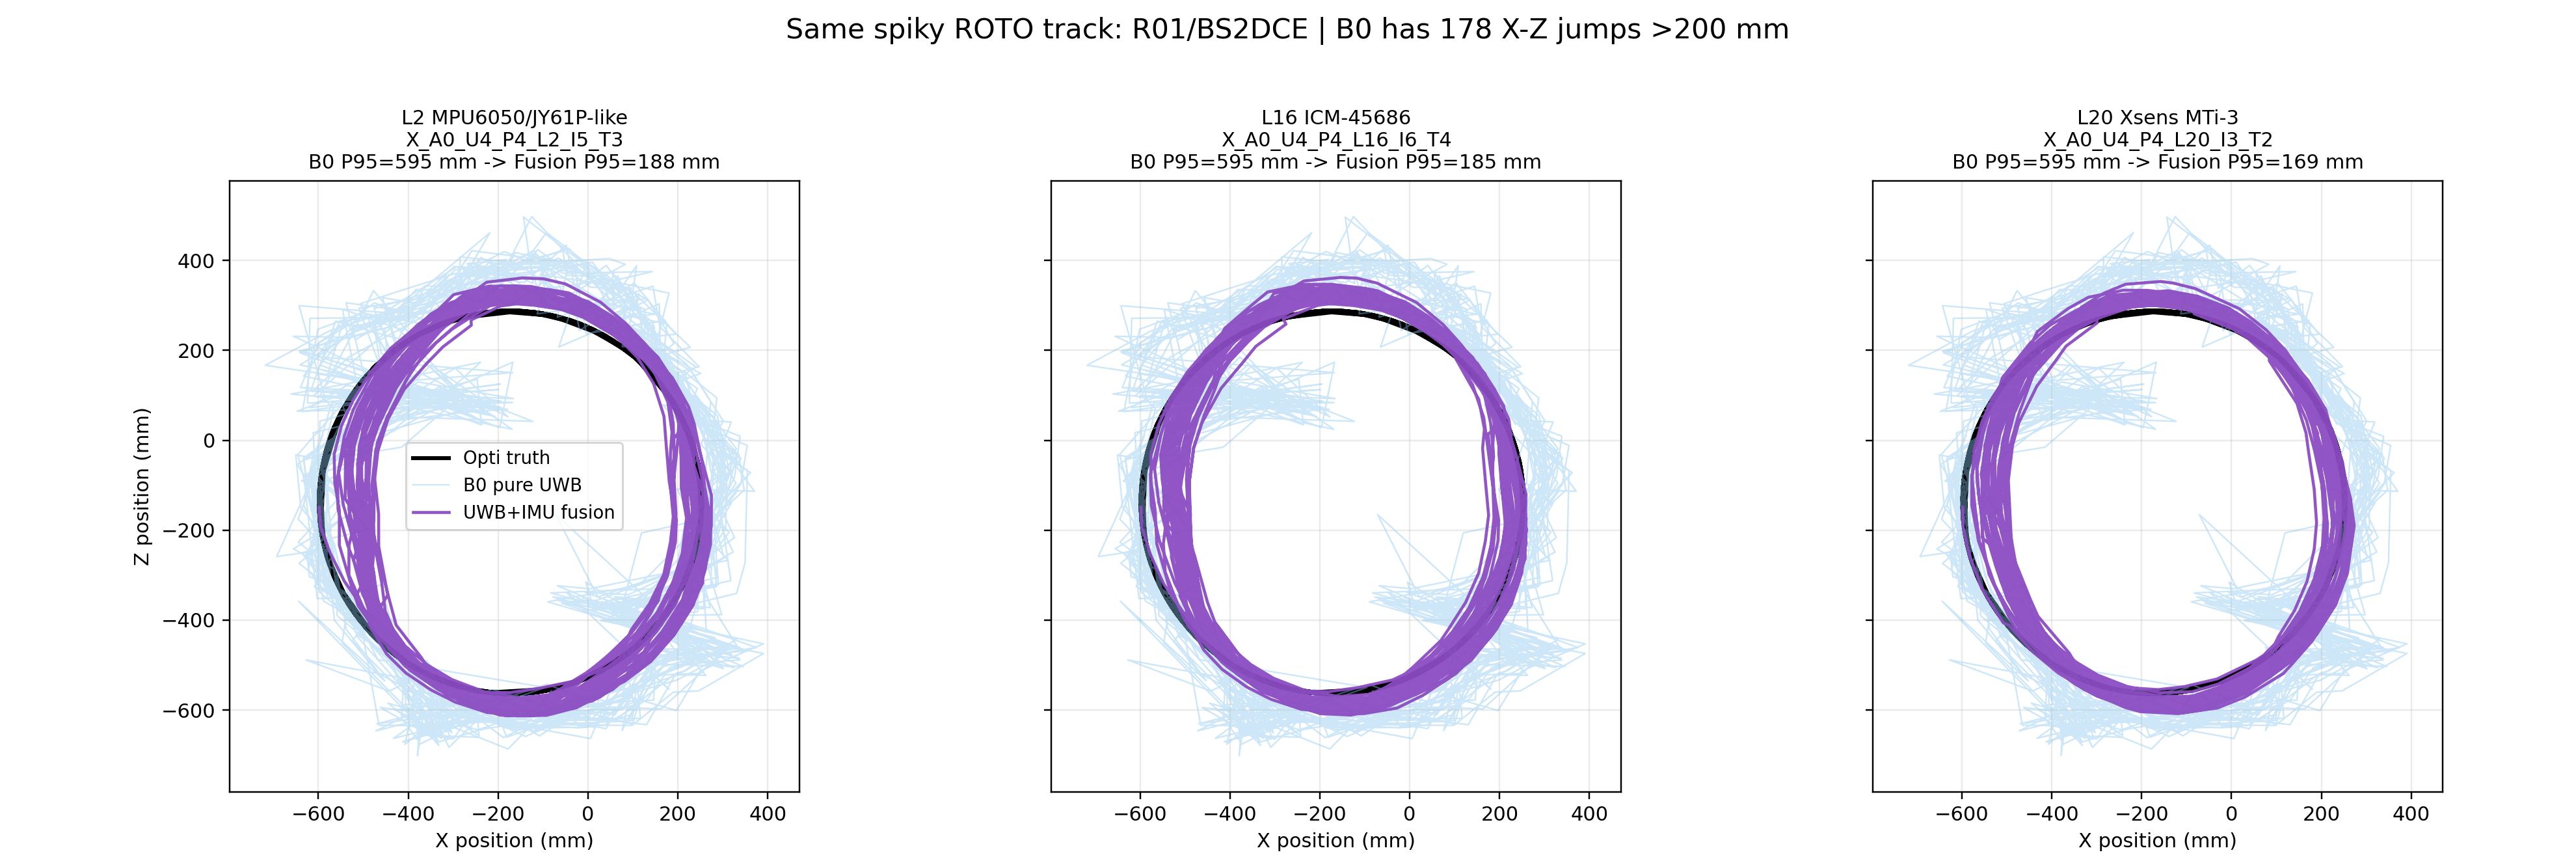
\includegraphics[width=0.82\textwidth]{phase4_spiky_track_xz_l2_l16_l20.png}
\caption{教授视角 spiky track：同一条 \case{R01/BS2DCE} 轨迹上 L2/L16/L20 的 X-Z 平面对比。该 track 被选择是因为 B0 pure UWB 在 RotoArm UWB-Tag set 中有最多 X-Z jump spikes。}
\end{figure}

\begin{figure}[H]
\centering
\begin{subfigure}{0.49\textwidth}
\centering
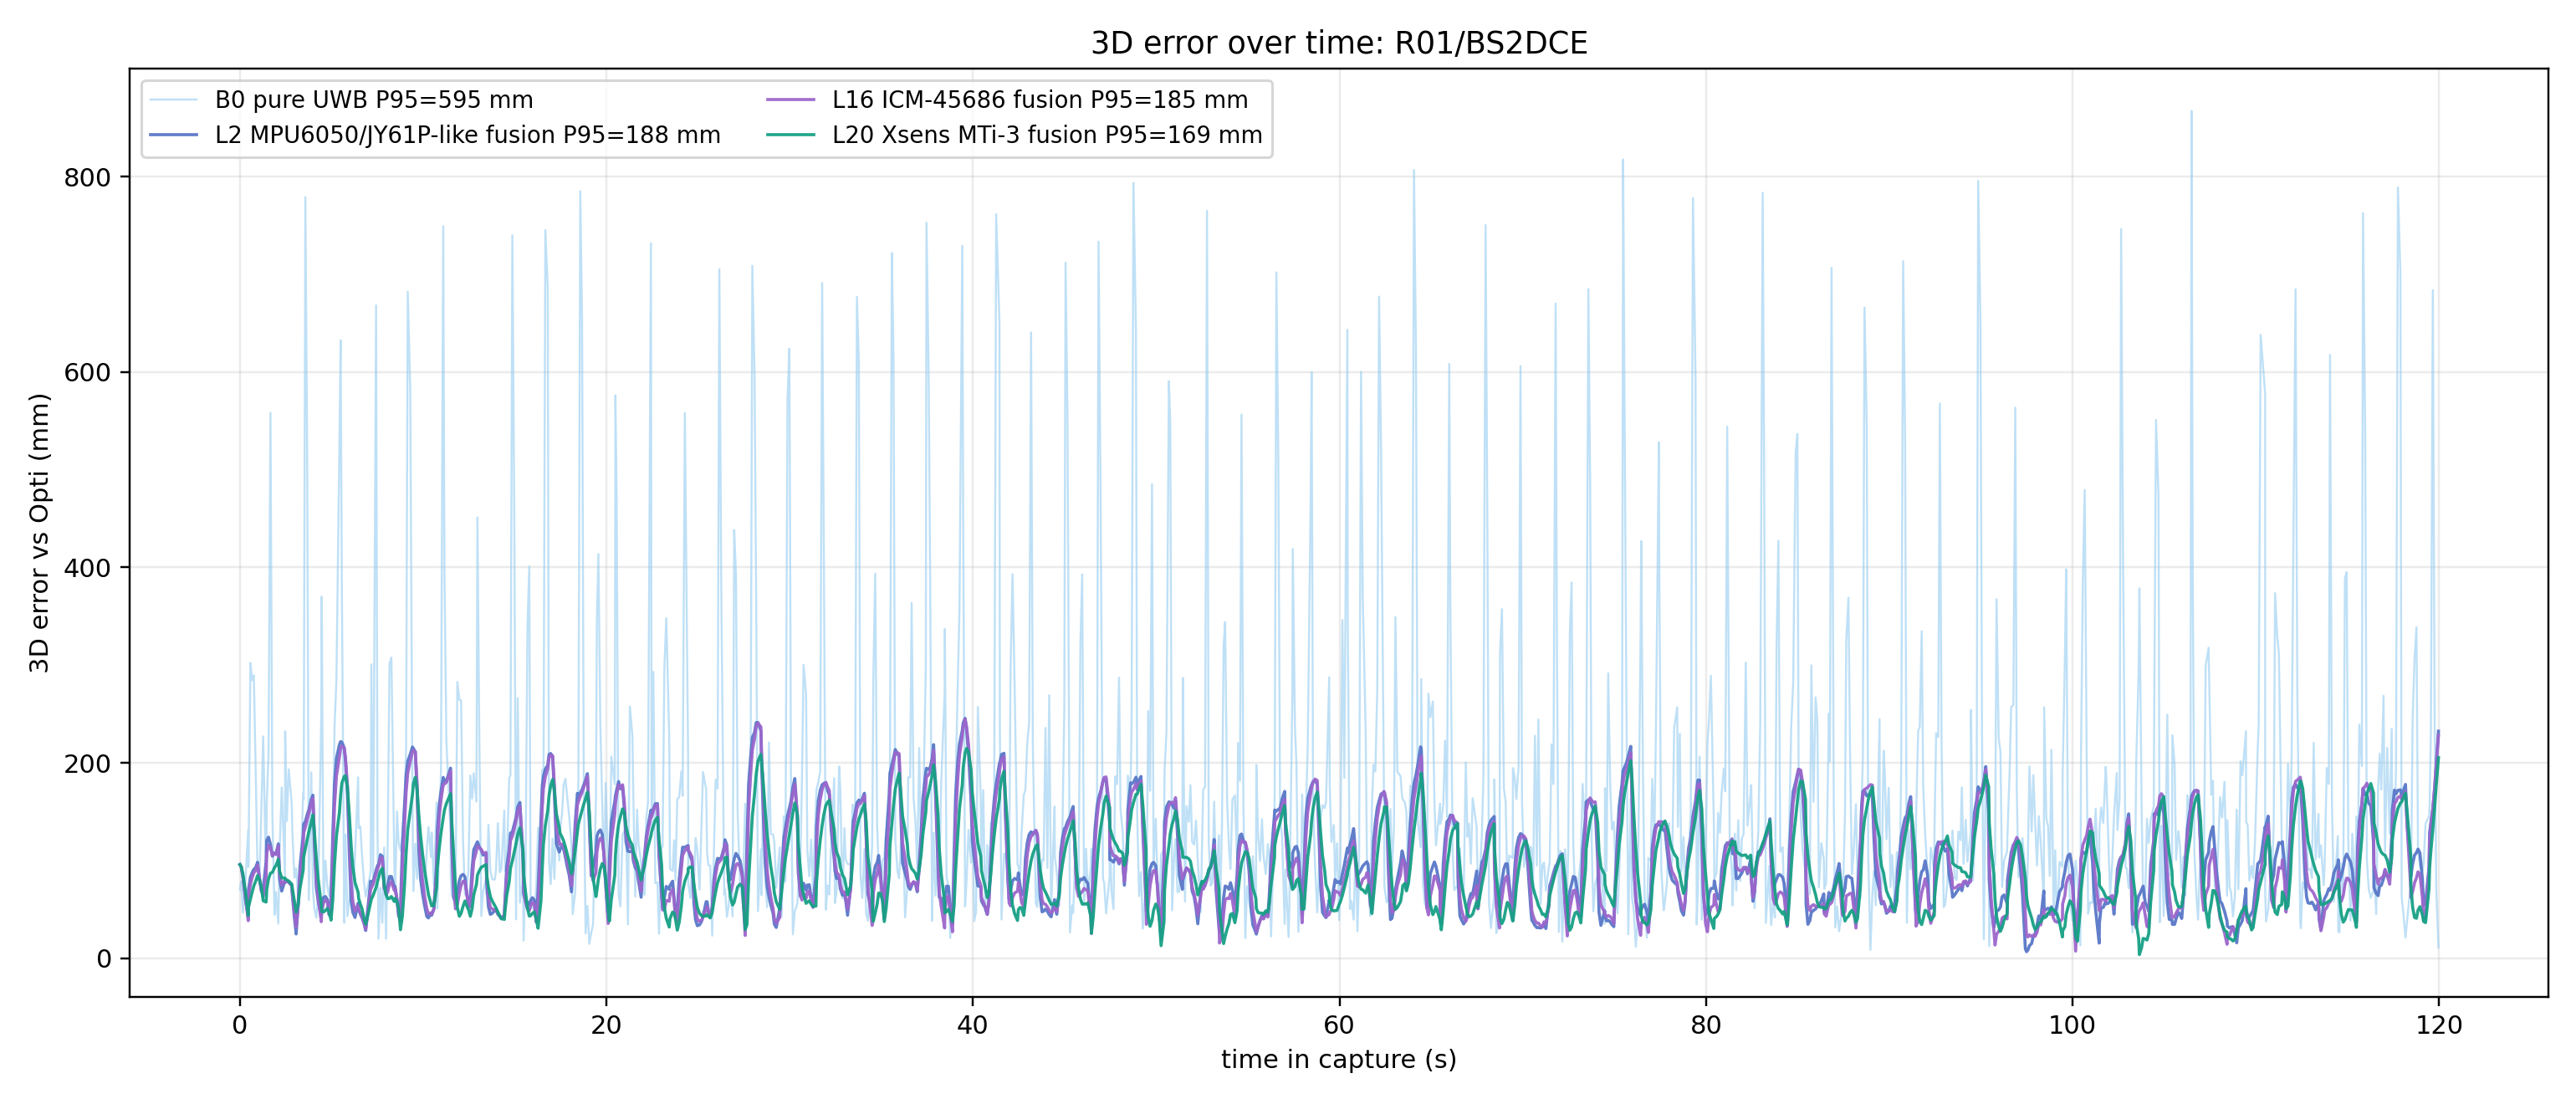
\includegraphics[width=\textwidth]{phase4_spiky_track_err3d_l2_l16_l20.png}
\caption{3D error over time}
\end{subfigure}
\begin{subfigure}{0.49\textwidth}
\centering
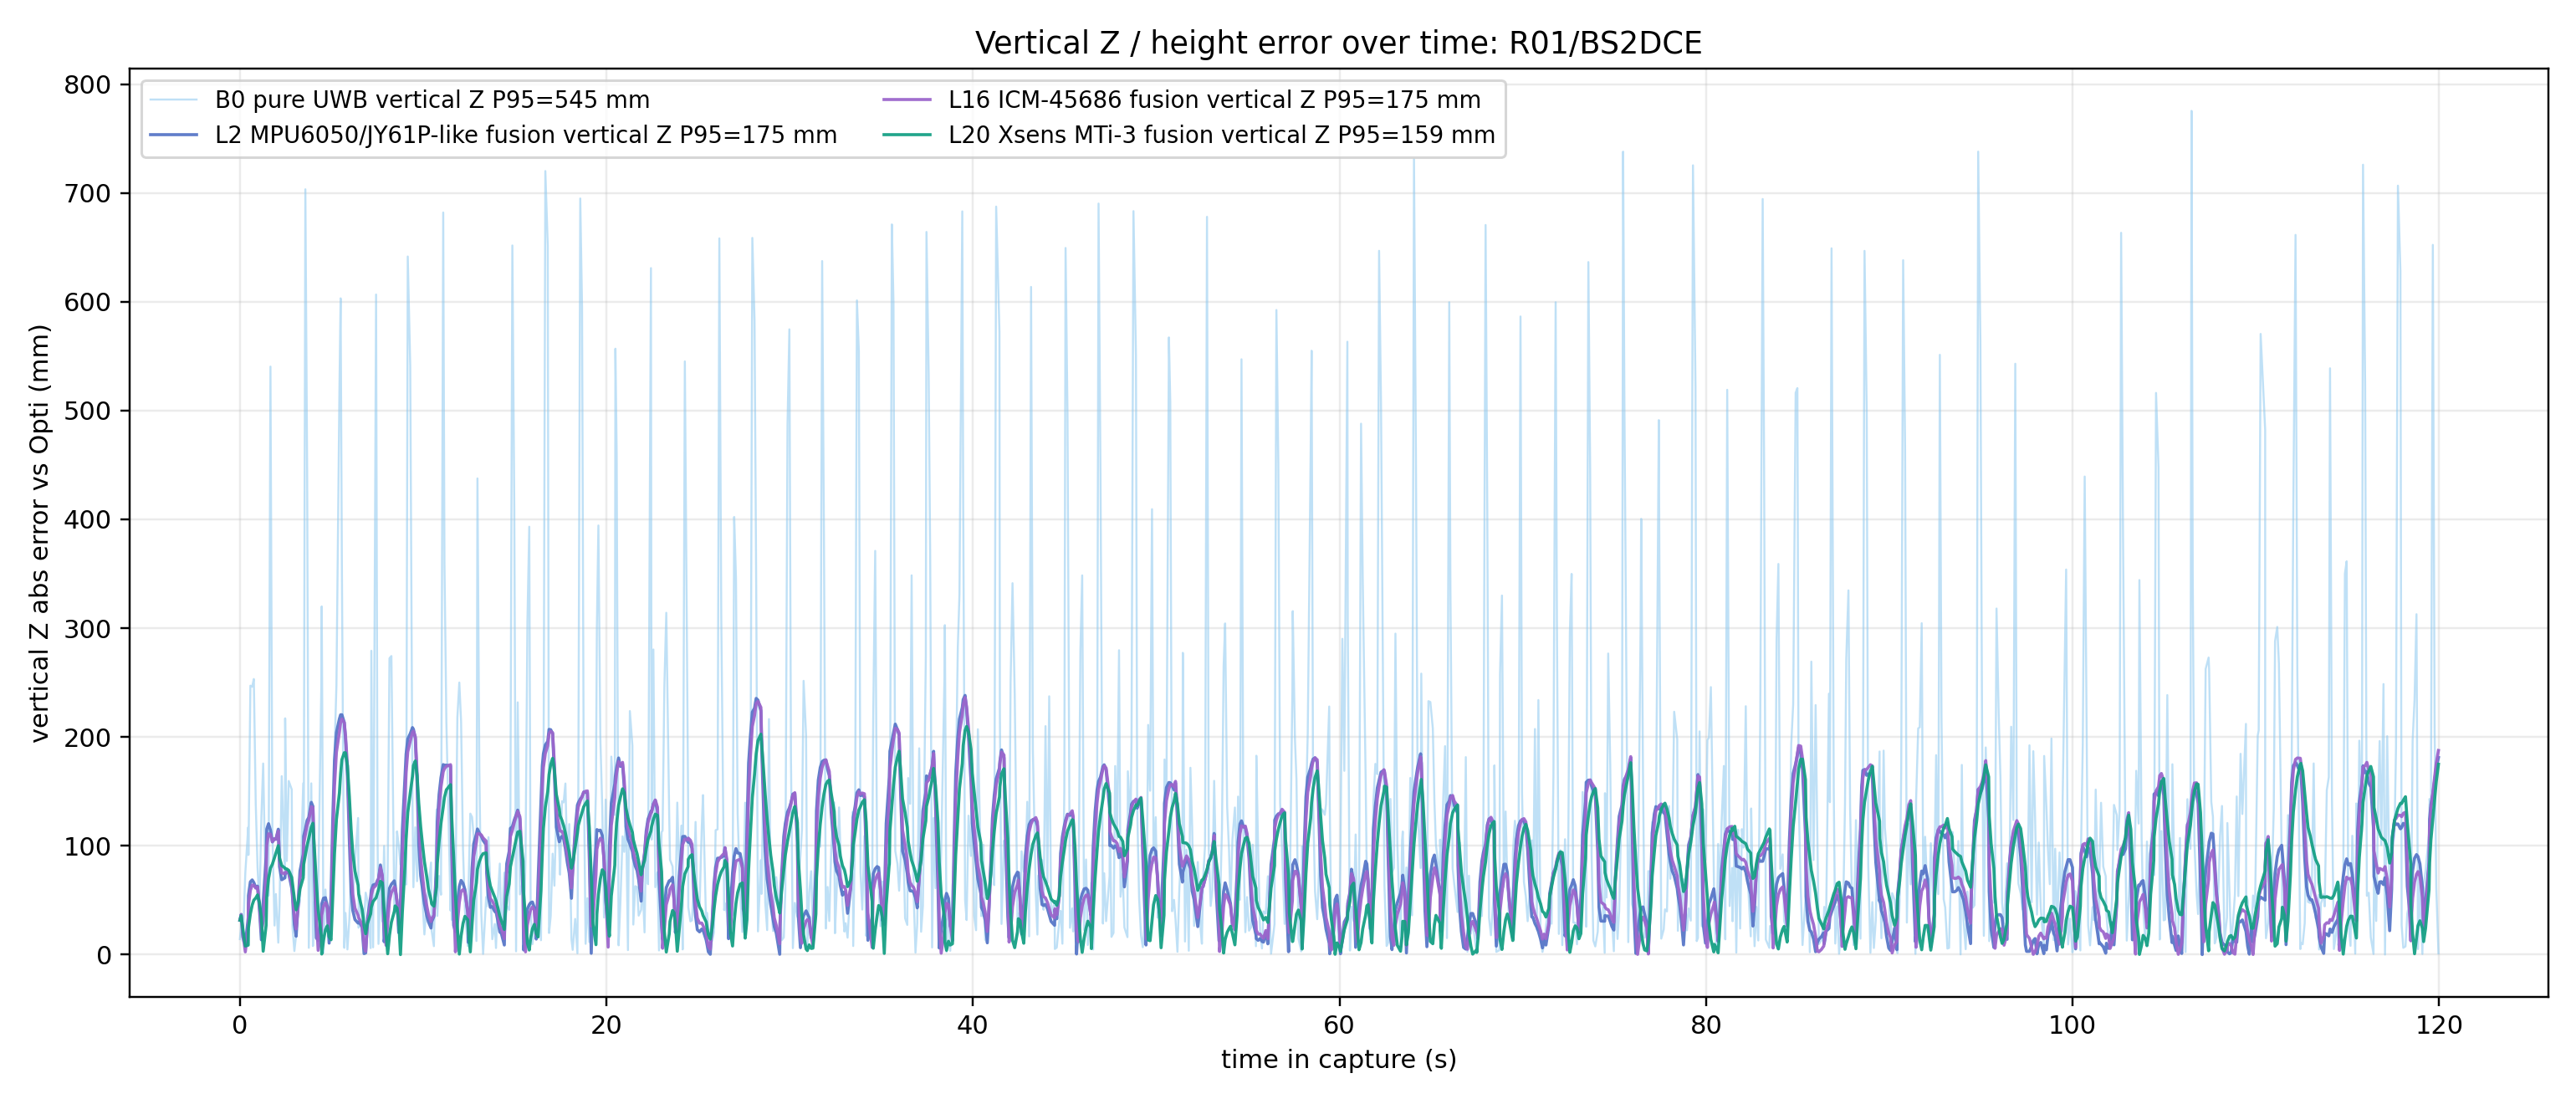
\includegraphics[width=\textwidth]{phase4_spiky_track_vertical_l2_l16_l20.png}
\caption{Vertical Z error over time}
\end{subfigure}
\caption{同一条 spiky track 的误差时间序列。这里 height axis 在图中写作 Vertical Z，内部使用 official aligned table 的 \case{y_vertical} height column。}
\end{figure}

教授视角的 spiky track 对报告很有价值，因为它不是只给 aggregate number，而是展示 IMU 到底救了什么。选中的 \case{R01/BS2DCE} 上，B0 pure UWB 有 178 个 X-Z jump $>200\mm$ 的采样点，jump p99 为 $425.8\mm$，max jump 为 $506.5\mm$，B0 3D P95 为 $595.5\mm$，B0 vertical Z P95 为 $545.1\mm$。加入三类 IMU 后，三条 fusion 轨迹的 X-Z jump $>200\mm$ count 都降到 0：
\begin{itemize}
\item \case{L2}: \case{X_A0_U4_P4_L2_I5_T3}，Fusion 3D P95 为 $188.4\mm$，相对 B0 改善 $407.0\mm$，Vertical Z P95 为 $175.4\mm$。
\item \case{L16}: \case{X_A0_U4_P4_L16_I6_T4}，Fusion 3D P95 为 $185.1\mm$，相对 B0 改善 $410.4\mm$，Vertical Z P95 为 $175.1\mm$。
\item \case{L20}: \case{X_A0_U4_P4_L20_I3_T2}，Fusion 3D P95 为 $169.4\mm$，相对 B0 改善 $426.0\mm$，Vertical Z P95 为 $159.3\mm$。
\end{itemize}

这部分建议在报告里写得更强一些：IMU fusion 的最大价值不是把每一个静态点变准，而是在动态 RotoArm UWB-Tag 中抑制 UWB-only 的离散跳变和 vertical spike。即使 L2 在 aggregate matched-best 表里不如 L16/L20，它在这条 spiky track 上仍能把大跳变全部压掉，说明低成本 IMU 对动态鲁棒性仍有工程价值。

\subsection{Stress test：稳健性排序}

\begin{figure}[H]
\centering
\begin{subfigure}{0.49\textwidth}
\centering
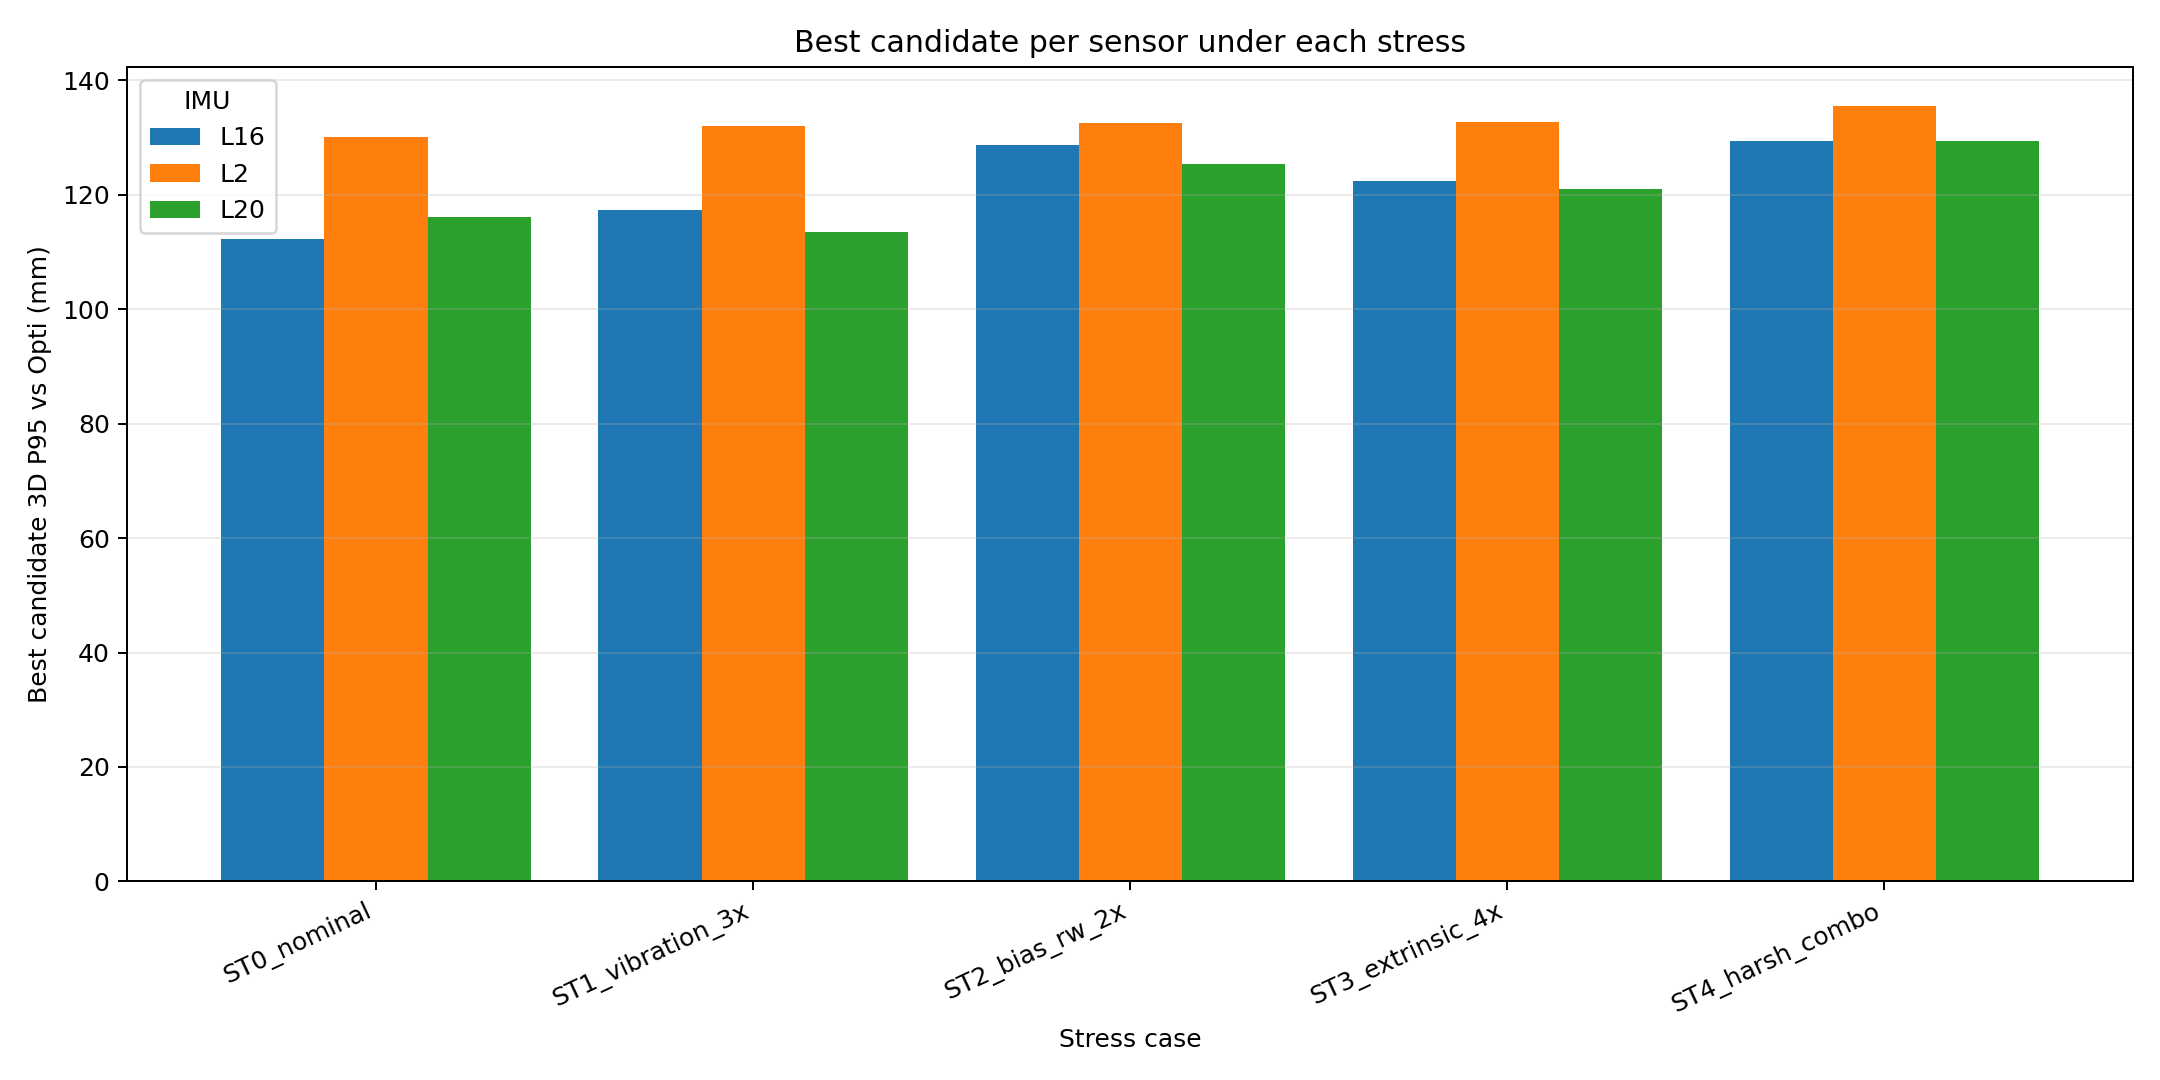
\includegraphics[width=\textwidth]{imu_stress_best_per_sensor_p95.png}
\caption{Best row per sensor and stress}
\end{subfigure}
\begin{subfigure}{0.49\textwidth}
\centering
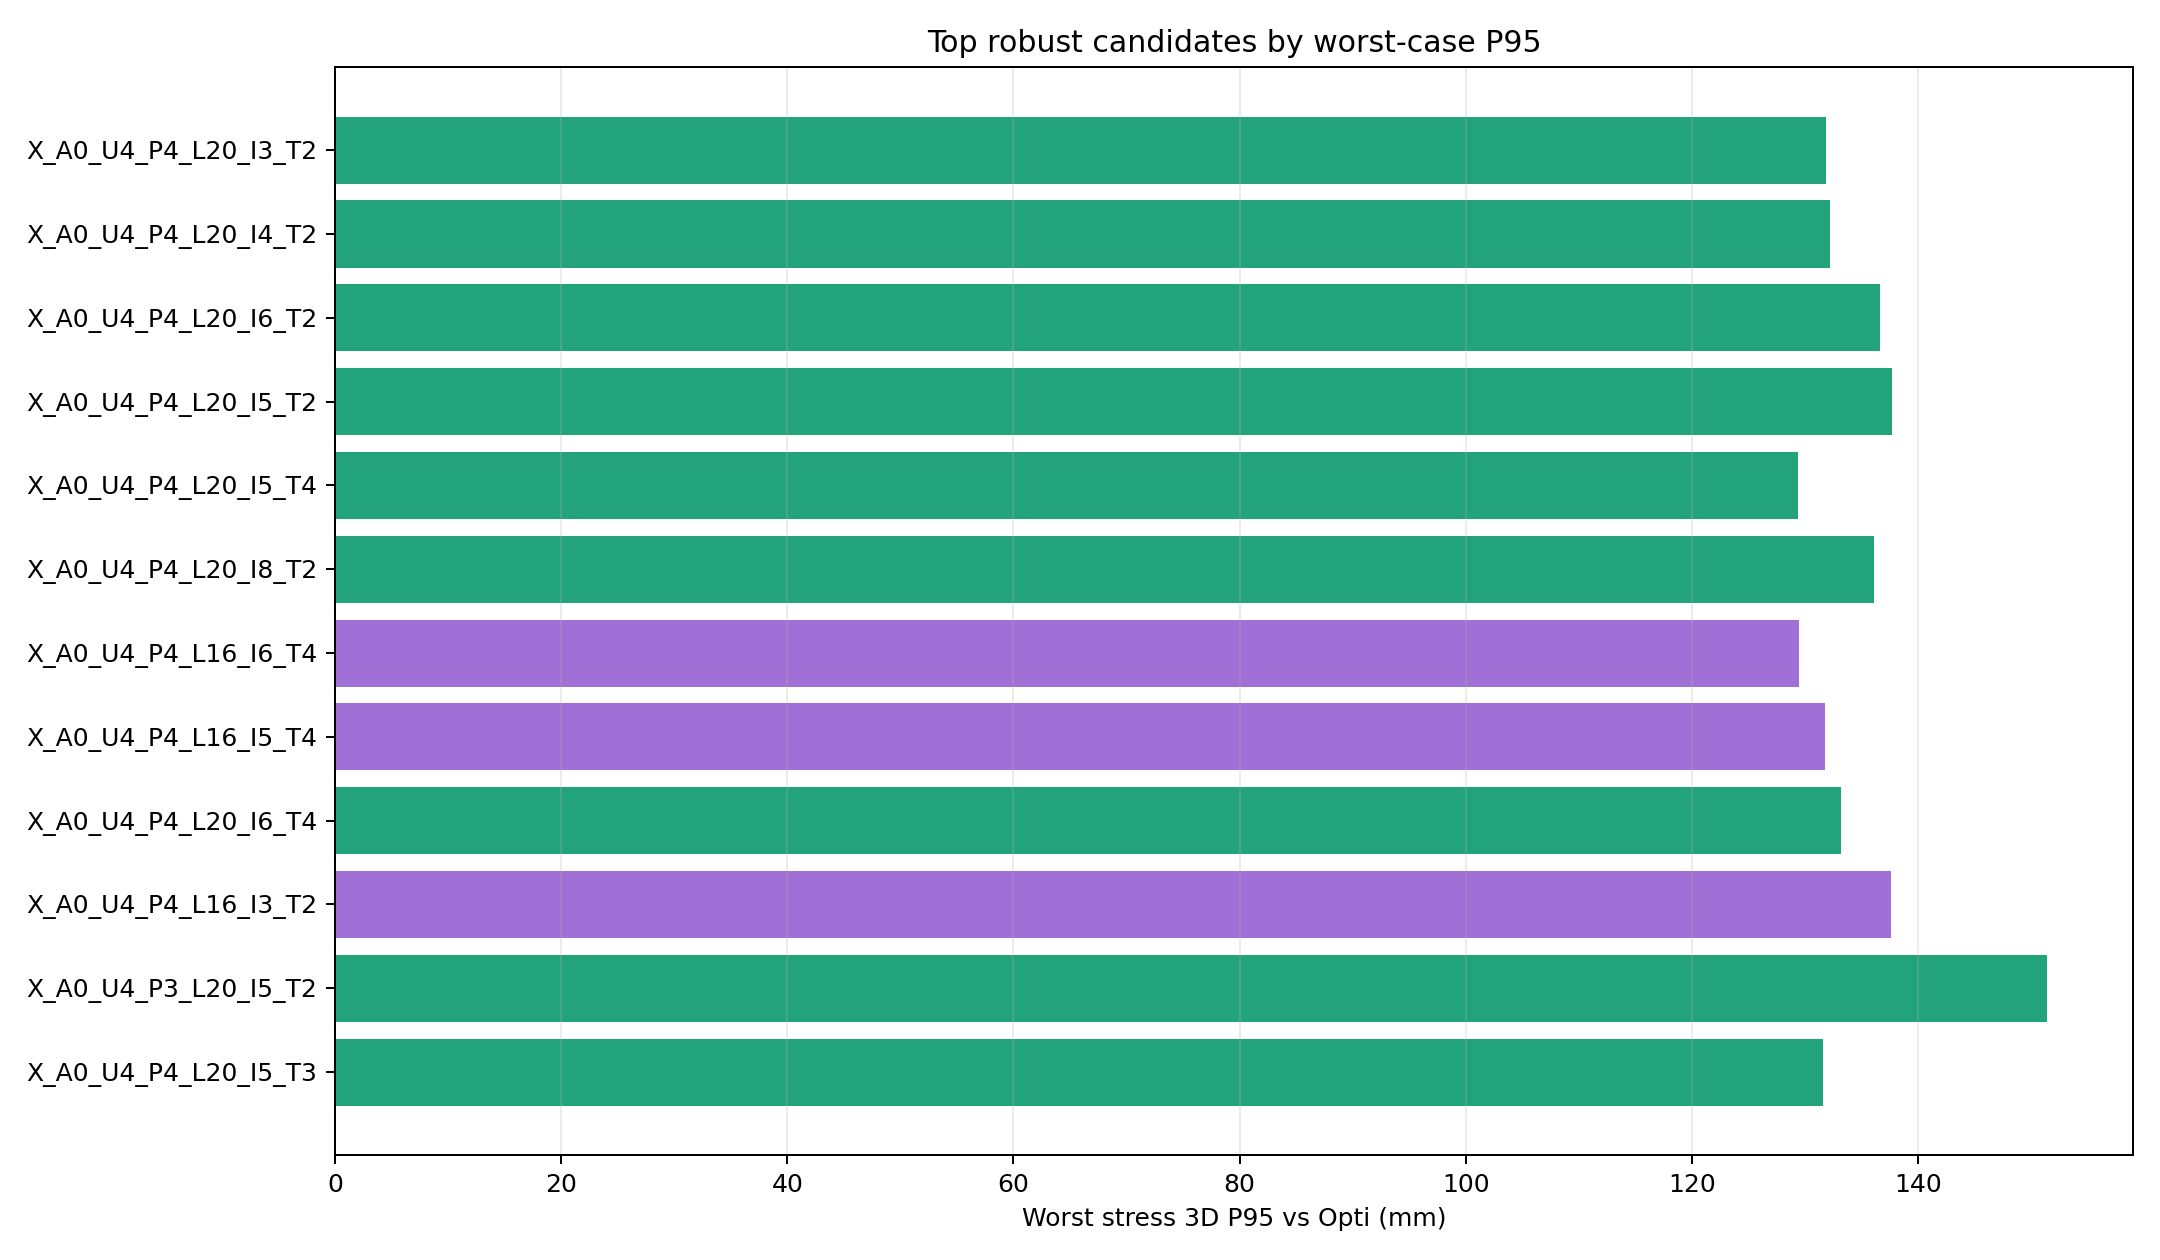
\includegraphics[width=\textwidth]{phase4_stress_top12_worstcase_p95.png}
\caption{Top12 worst-case P95 ranking}
\end{subfigure}
\caption{Phase 4 L2/L16/L20 stress candidate test。Stress cases 包括 vibration、bias random walk、extrinsic 和 harsh combo。}
\end{figure}

Stress candidate test 使用五种 stress case：\case{ST0_nominal}、\case{ST1_vibration_3x}、\case{ST2_bias_rw_2x}、\case{ST3_extrinsic_4x}、\case{ST4_harsh_combo}。最稳健的前几名几乎都来自 L20；robust rank 1 是 \case{X_A0_U4_P4_L20_I3_T2}，mean P95 为 $124.1\mm$，worst P95 为 $131.9\mm$，same-P mean improvement 为 $14.8\mm$。L16 最好的 robust row 排名第 7，为 \case{X_A0_U4_P4_L16_I6_T4}，mean/worst P95 为 $129.1/129.5\mm$。L2 在各 stress 下通常落后，但 worst-case 仍保持在约 $130$--$136\mm$ P95 区间，说明低成本 IMU 的问题主要是上限不如 L16/L20，而不是完全不可用。

这一节应该给出非常明确的工程判断：如果目标是最佳动态性能和 stress robustness，L20/Xsens-like 工业 IMU 是当前 Phase 4 winner；如果考虑成本、体积和可采购性，L16/ICM-45686 与 L20 非常接近，是更现实的高性能 6-axis candidate；L2/MPU6050-like 适合作为低成本 baseline，它在 aggregate precision 上弱一些，但对极端 UWB spike 仍有明显 rescue 价值。

\subsection{Raw-range branch 当前不能推荐}

Phase 4 还测试了 raw-range branch，但报告中必须写清楚当前 proxy implementation 不推荐。最佳 raw row \case{X_A0_R4_L20_I5_T10} 的 P95 为 $465.4\mm$，相对 B0 的 delta 为 $-233.6\mm$，也就是显著变差。这说明当前 UWB+IMU 的有效路径是 position branch \case{A0/U4/Px} 上的 fusion，而不是直接把 raw range branch 当作最终算法。

\subsection{IMU 结论与边界}

IMU 现在不应该只写成 future work。更准确的写法是：\textbf{UWB+IMU 已经有 Phase 4 级别的仿真/重放证据，能够降低 RotoArm UWB-Tag P95、抑制 spiky jumps，并在 stress test 中区分不同 IMU sensor model 的工程价值。} 但它仍不应抢走 Vicon Motion Capture System--UWB 主报告的中心位置，因为当前 Phase 4 仍是 Vicon-truth evaluation 和 simulated sensor model sweep，不等同于完全实时、完全嵌入式闭环的 Ghost IMU 系统实测。主报告可以把 IMU 放在动态扩展结果或 discussion 的后半部分，明确说它是下一阶段最有希望进入系统的方向。

\section{CIR：clear LOS 下仍存在 multipath 证据}

CIR 不应只写成 future work。更准确的定位是：\textbf{CIR 目前不是完整的 LOS/NLOS 分类器结果，但已经能作为真实传播现象的证据，解释为什么看起来 clear LOS 的 anchor self-calibration 仍可能出现 multipath、tail energy 和链路质量差异。} 这部分应该作为误差来源分析章节，而不是作为主定位精度 headline。

本报告使用两类 CIR 结果：
\begin{itemize}
\item \textbf{FULL CIR Sweep10：}目录为 \case{CIRRAW_AUTOPOS_SWEEP10_20260602_225118}。该实验在 AutoPos Sweep10 中采集 full accumulator，重建 958 个完整 full-CIR frames，预期约 1120 个，覆盖率为 85.5\%。每个 accumulator 为 4064 bytes，即 1016 complex samples。
\item \textbf{F/H 8 小时 FULL CIR baseline：}目录为 \case{CIRRAW_BSF66F_20260602_020301}。该实验只采 F/H priority full CIR，持续 8.00 h，共 31,514 frames，用于观察稳定链路在长时间 clear/static 条件下的 waveform 和 tail/main 分布。
\end{itemize}

\begin{figure}[H]
\centering
\begin{subfigure}{0.49\textwidth}
\centering
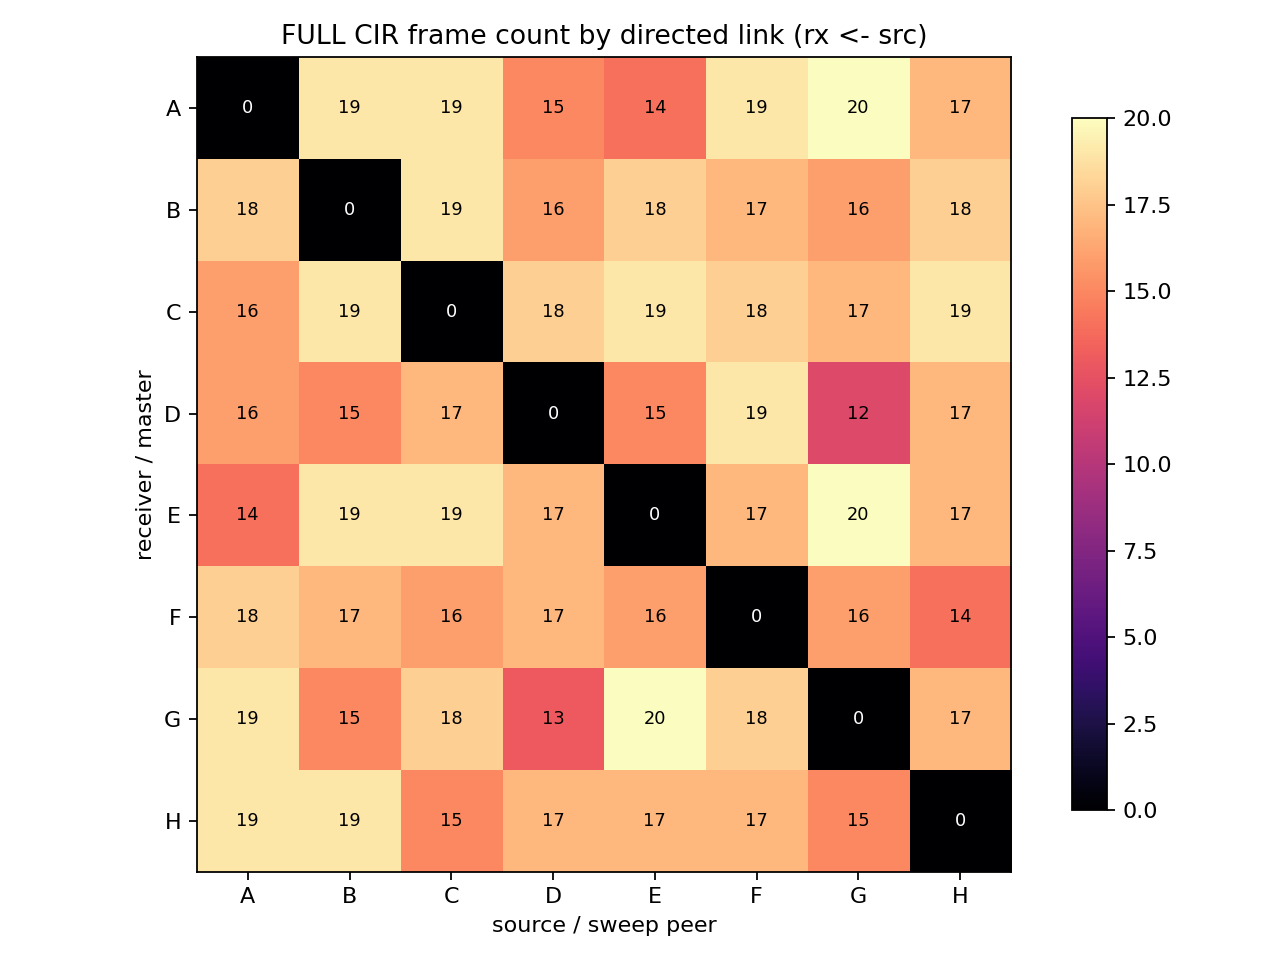
\includegraphics[width=\textwidth]{cir_full_frame_count_heatmap.png}
\caption{FULL CIR frame count}
\end{subfigure}
\begin{subfigure}{0.49\textwidth}
\centering
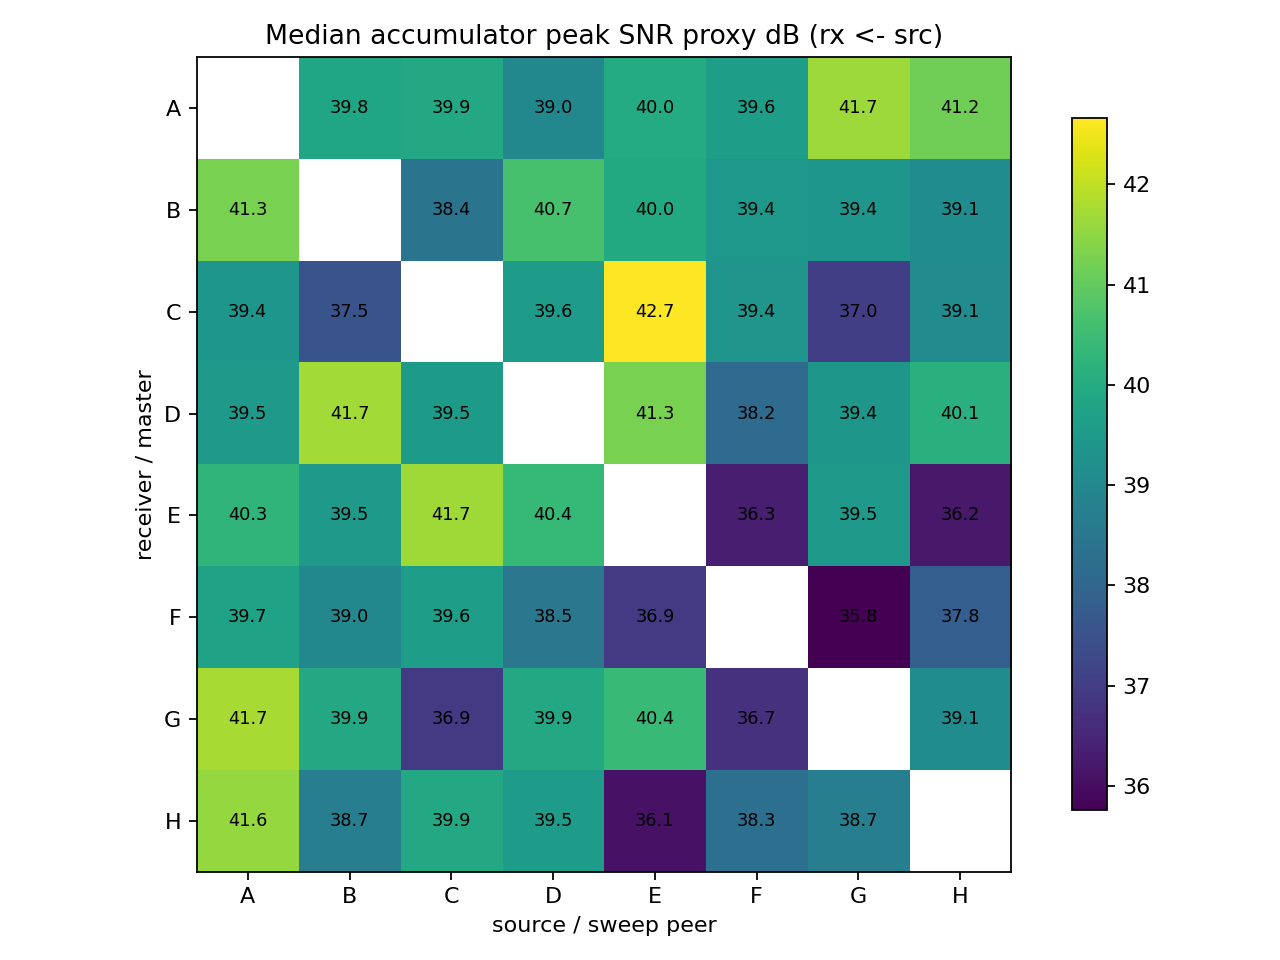
\includegraphics[width=\textwidth]{cir_full_snr_proxy_heatmap.png}
\caption{SNR proxy}
\end{subfigure}
\caption{FULL CIR Sweep10 的覆盖和 SNR proxy。该结果说明 full accumulator over USB 可以工作，但全锚点 full-CIR 对 USB/CDC 带宽压力很大，不能直接当成 Sweep1000 的默认采集模式。}
\end{figure}

\begin{figure}[H]
\centering
\begin{subfigure}{0.49\textwidth}
\centering
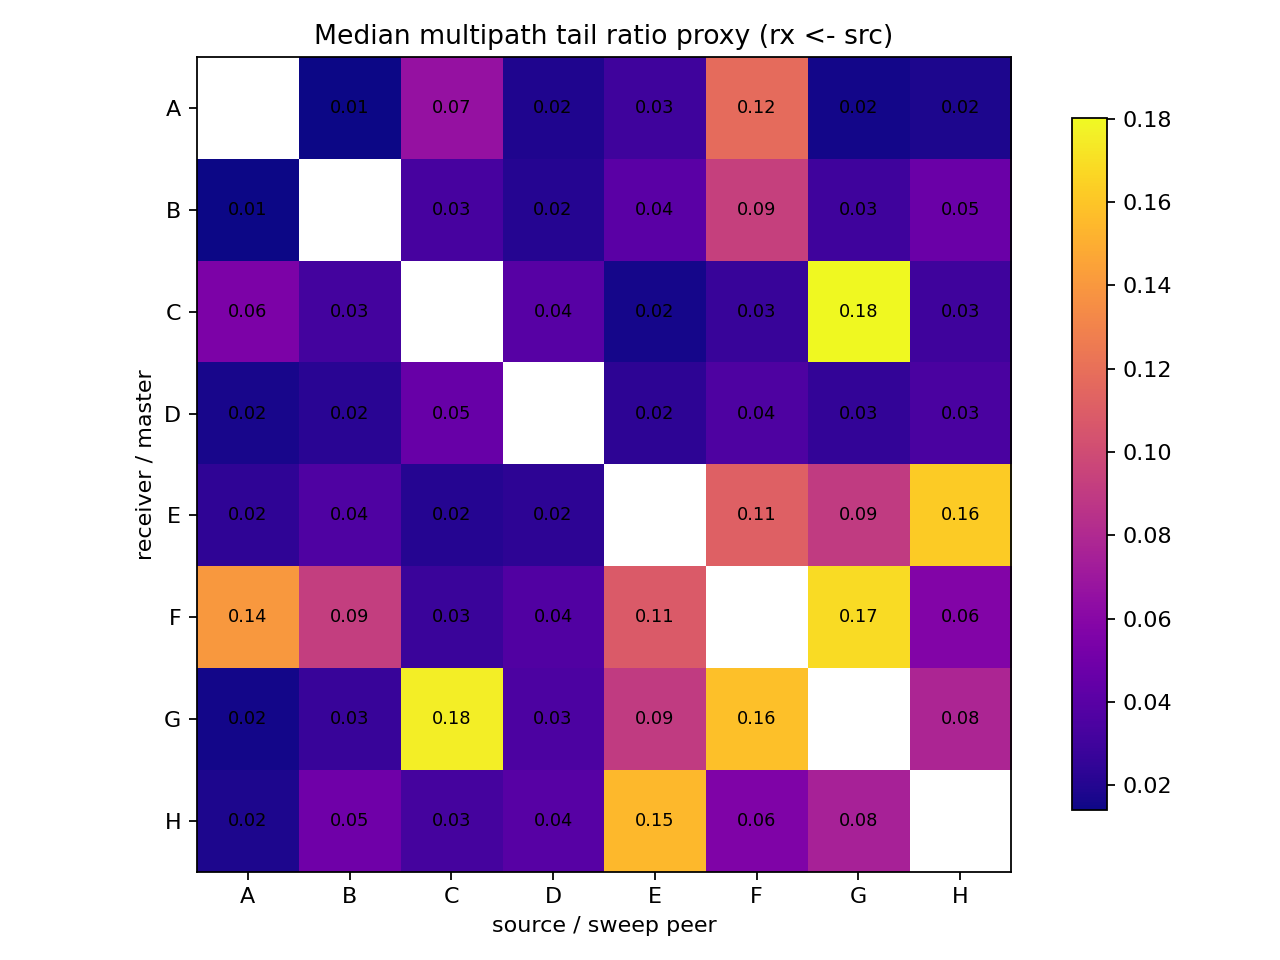
\includegraphics[width=\textwidth]{cir_full_tail_ratio_heatmap.png}
\caption{Tail/main proxy by directed link}
\end{subfigure}
\begin{subfigure}{0.49\textwidth}
\centering
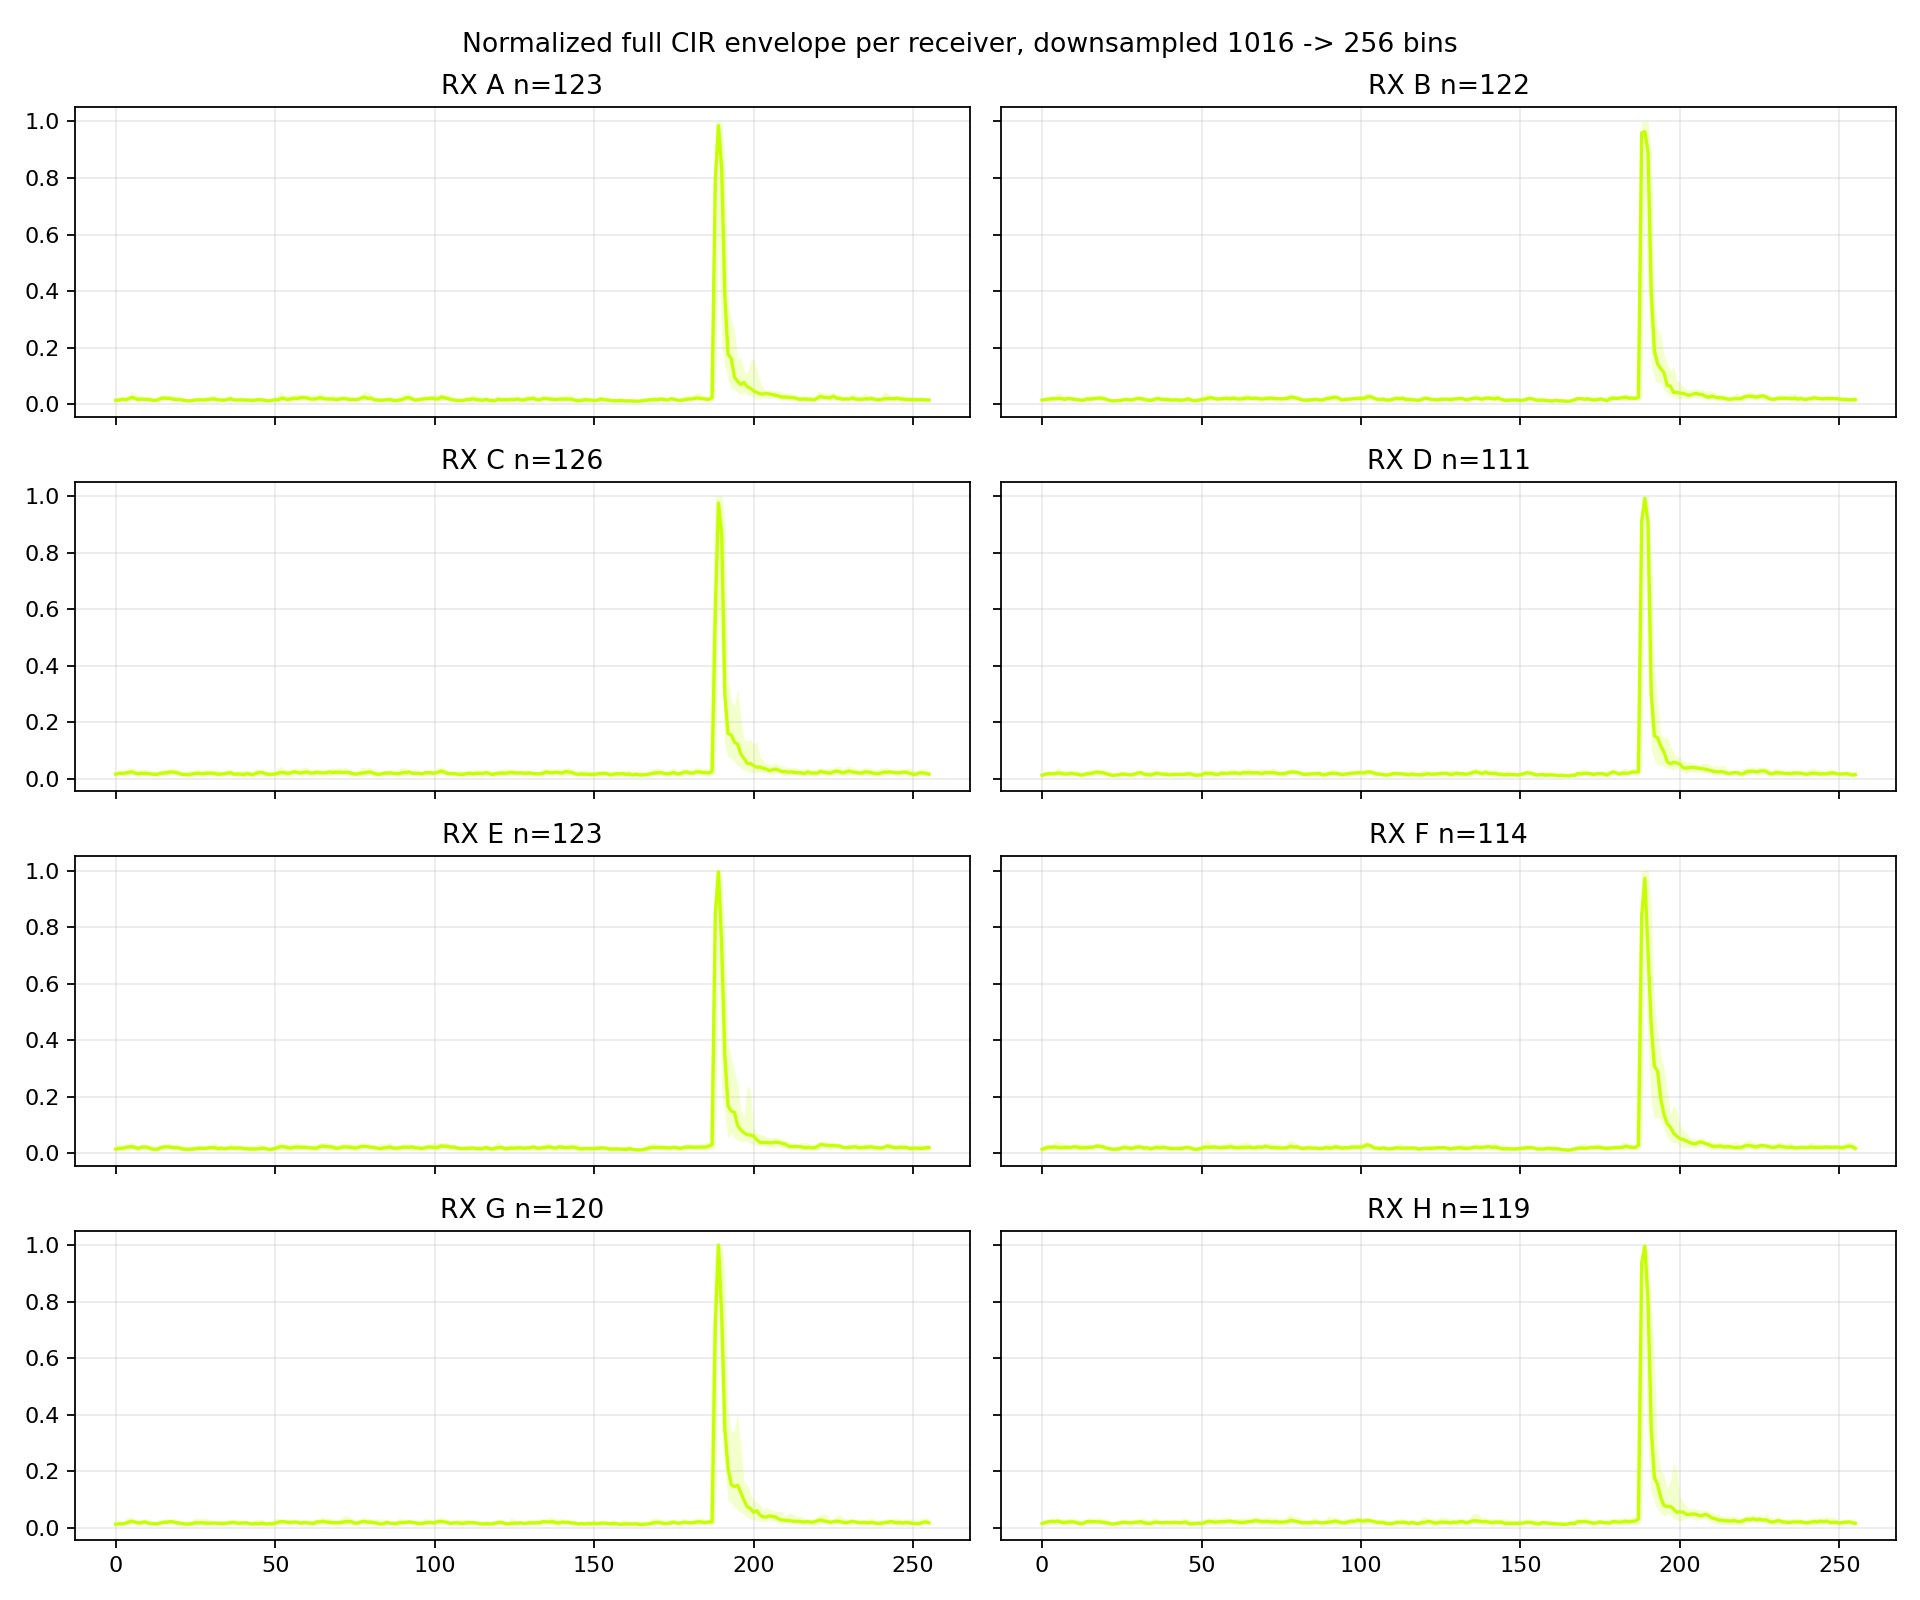
\includegraphics[width=\textwidth]{cir_full_receiver_envelope_overview.png}
\caption{Receiver envelope overview}
\end{subfigure}
\caption{FULL CIR 的 multipath-tail 证据。即使实验环境中多数 anchor 之间视觉上接近 clear LOS，不同 directed links 的 tail/main proxy 仍有明显差异。}
\end{figure}

FULL CIR Sweep10 的主要事实是：8/8 masters 成功，每个 master 完成 $10/10$ sweep lines，普通 ranging 本身正常；但 full-CIR 的 link-level 质量并不均匀。最高 multipath-tail proxy 的 directed links 包括 \case{C<-G}、\case{G<-C}、\case{F<-G}、\case{E<-H}、\case{G<-F}、\case{H<-E} 等，tail/main proxy 约为 0.2。弱 SNR-proxy links 也集中在部分 pair 上，例如 \case{F<-G}、\case{H<-E}、\case{E<-H}、\case{E<-F}、\case{G<-F}、\case{G<-C}。这说明 anchor self-calibration 里所谓 ``clear LOS'' 不能简化成 ``每条 range 都是单径、无偏、同方差''。

从物理上看，clear LOS 只表示直达路径存在，并不表示反射路径不存在。UWB 接收端仍会看到地面、墙面、金属结构、支架、人体或设备外壳引起的延迟能量。对于 anchor-anchor self-calibration，这些 multipath/tail 能量会表现为链路特定的 range bias 或 variance difference。它不会一定导致某条链路完全失效，但会让不同 pair 对 layout scale、delay fitting 和 residual distribution 的贡献不同。

\begin{figure}[H]
\centering
\begin{subfigure}{0.49\textwidth}
\centering
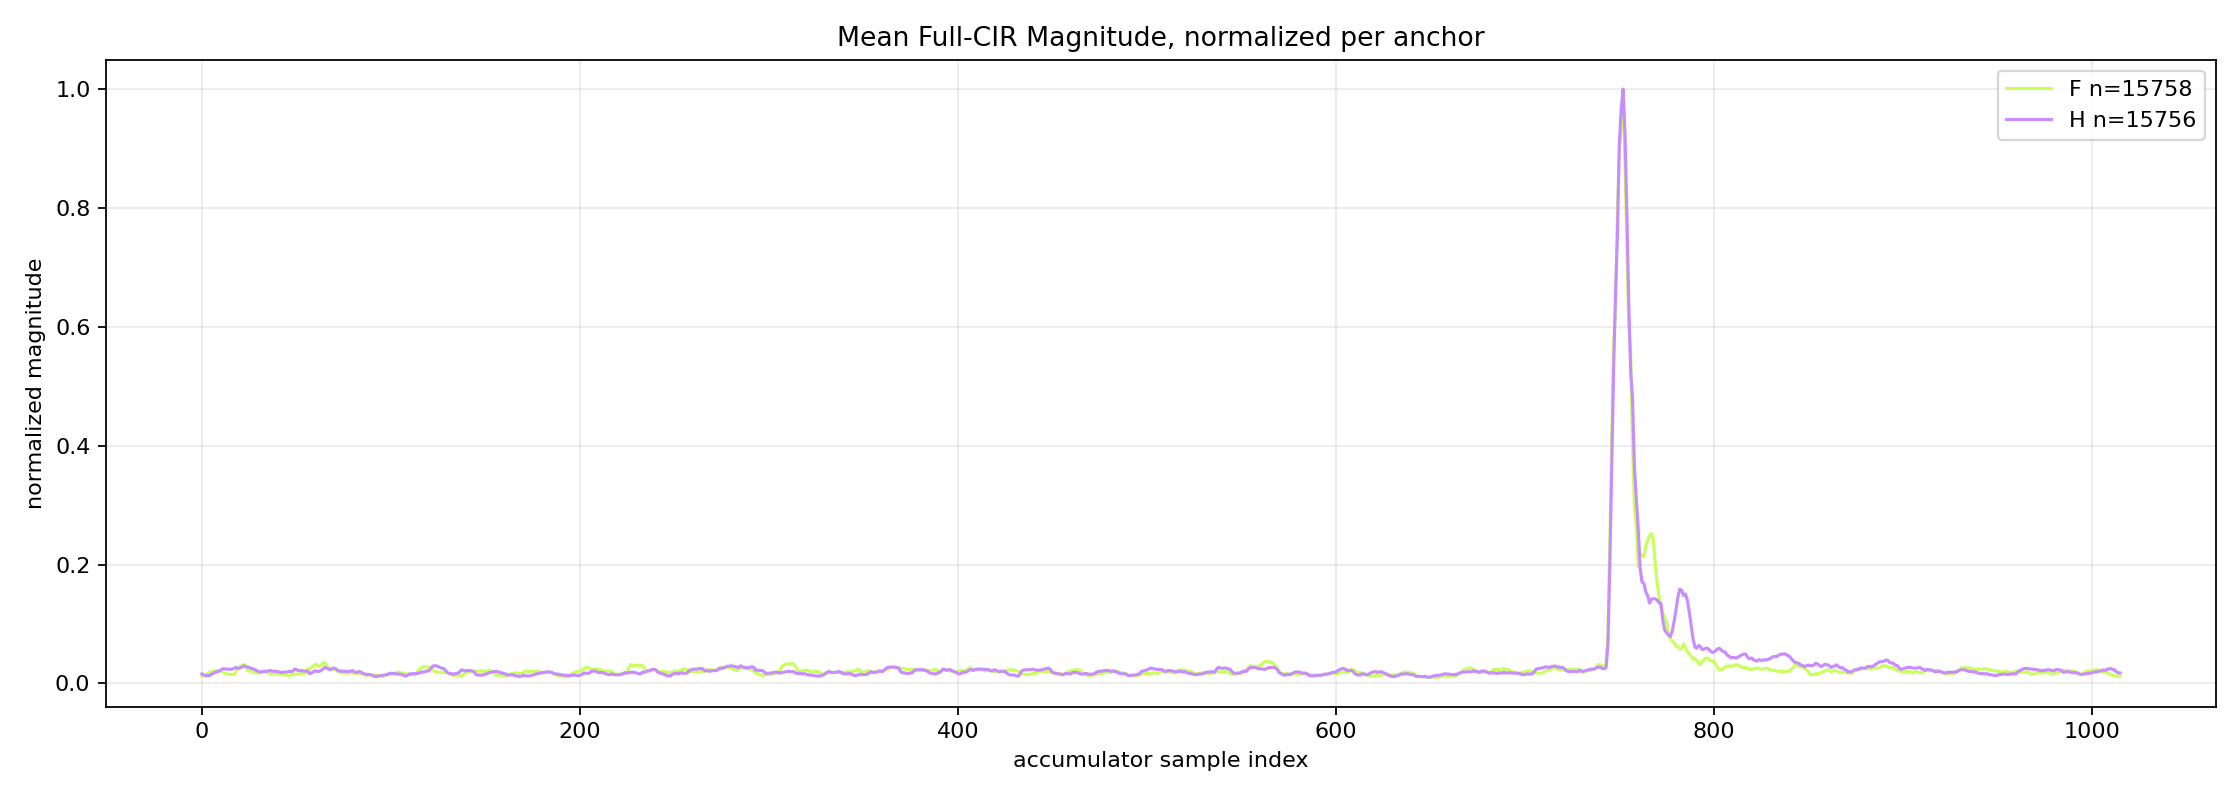
\includegraphics[width=\textwidth]{cir_fh_mean_waveforms.png}
\caption{F/H mean full-CIR waveforms}
\end{subfigure}
\begin{subfigure}{0.49\textwidth}
\centering
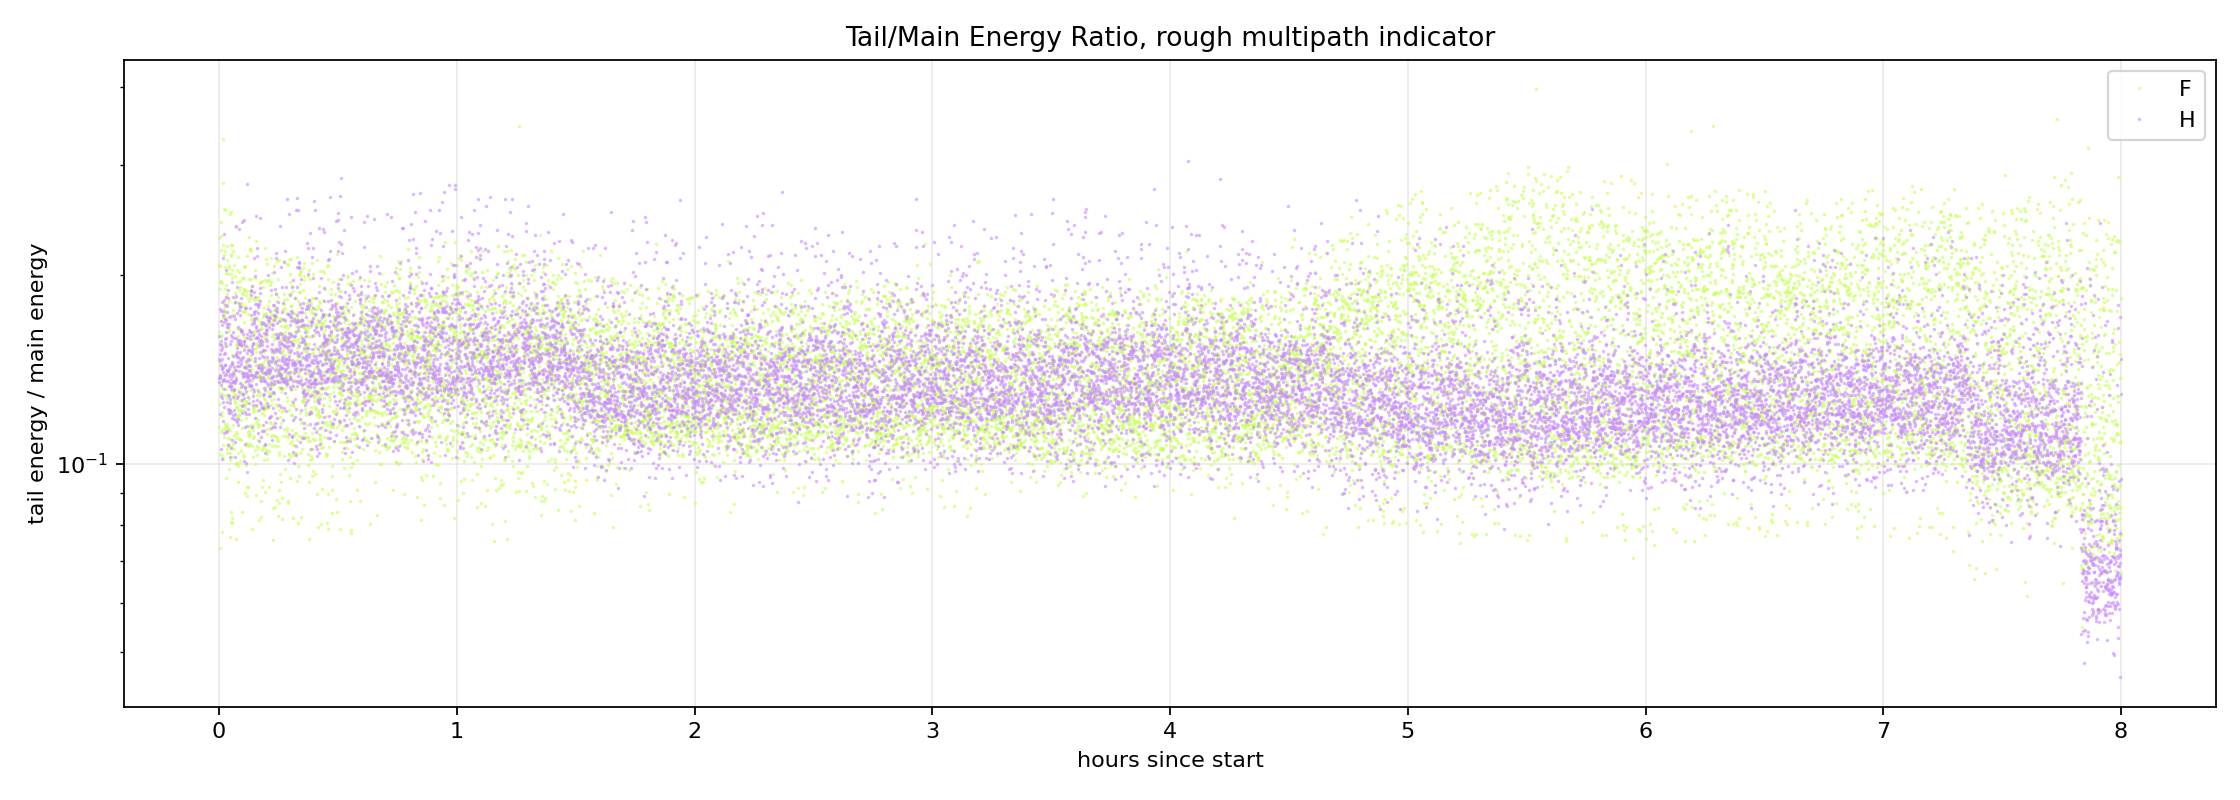
\includegraphics[width=\textwidth]{cir_fh_tail_ratio_timeseries.png}
\caption{F/H tail/main time series}
\end{subfigure}
\caption{F/H 8 小时 full-CIR baseline。该实验不是全锚点 sweep，而是为了避免 DW1000 single-accumulator overwrite/timing limit，只对 F/H priority link 做稳定长时间采集。}
\end{figure}

F/H 8 小时实验进一步说明，即使是稳定 priority-only capture，full-CIR waveform 中也有可测的 tail energy。F anchor 的 tail/main median 为 0.137，P95 为 0.215；H anchor 的 tail/main median 为 0.132，P95 为 0.186。两者的 peak index median 都约为 750，IQR 为 4，说明主峰位置稳定，但主峰后的 tail energy 仍长期存在。这个现象适合直接写进报告：\textbf{clear LOS 并不等价于理想单径；CIR 证据显示在 anchor self-calibration 中仍应考虑 multipath-tail 和链路质量权重。}

\subsection{COMPACT CIR：从现象证据到 pair weighting}

\begin{figure}[H]
\centering
\begin{subfigure}{0.49\textwidth}
\centering
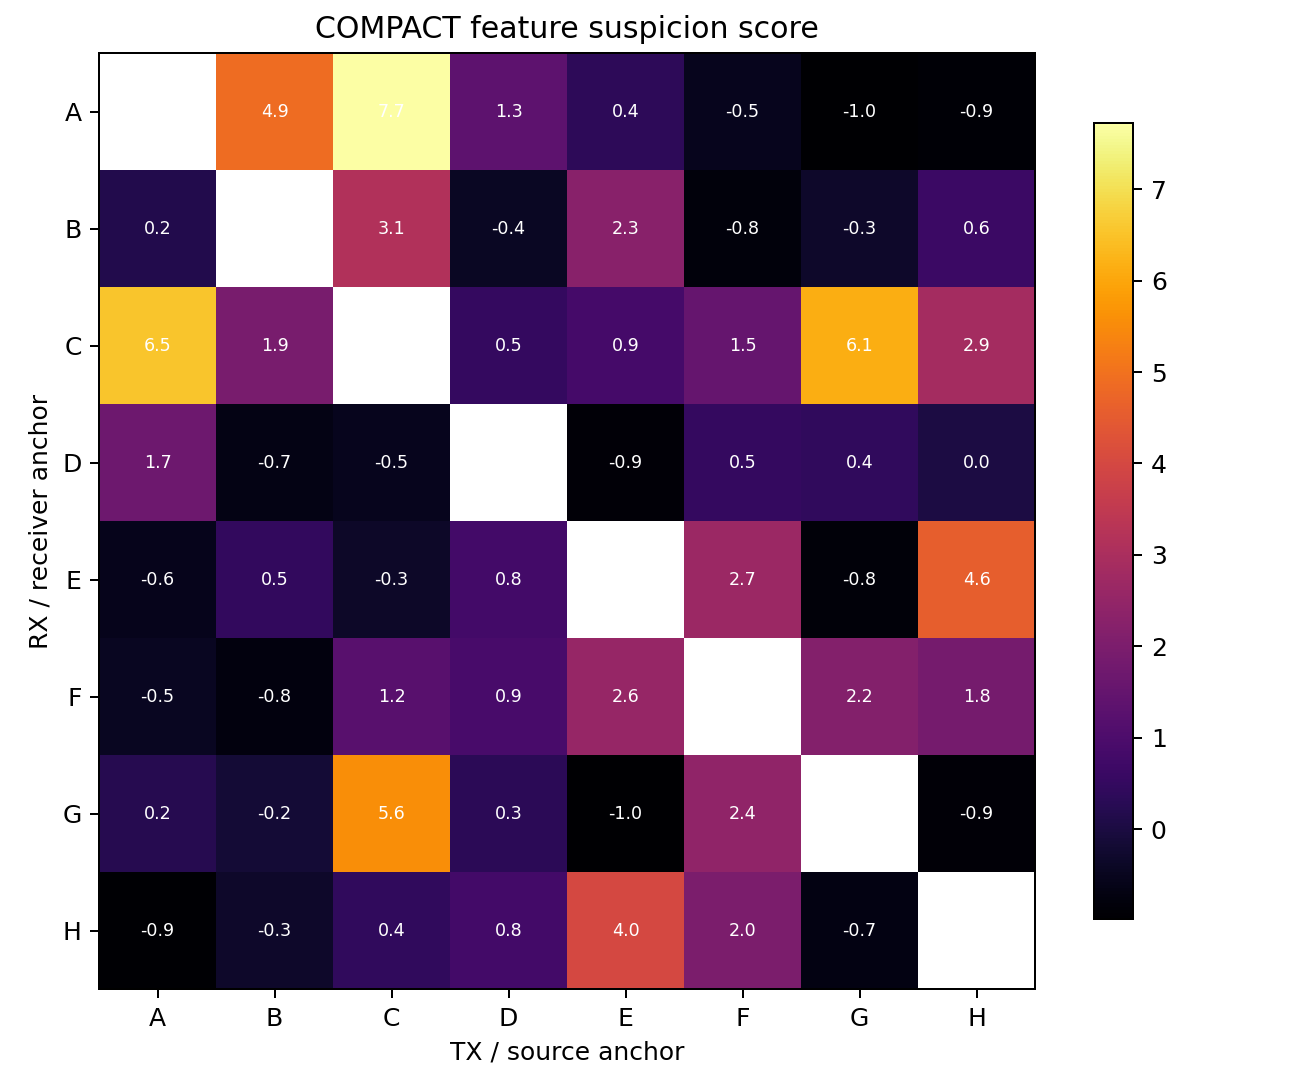
\includegraphics[width=\textwidth]{cir_compact_suspicion_score_heatmap.png}
\caption{Compact CIR suspicion score}
\end{subfigure}
\begin{subfigure}{0.49\textwidth}
\centering
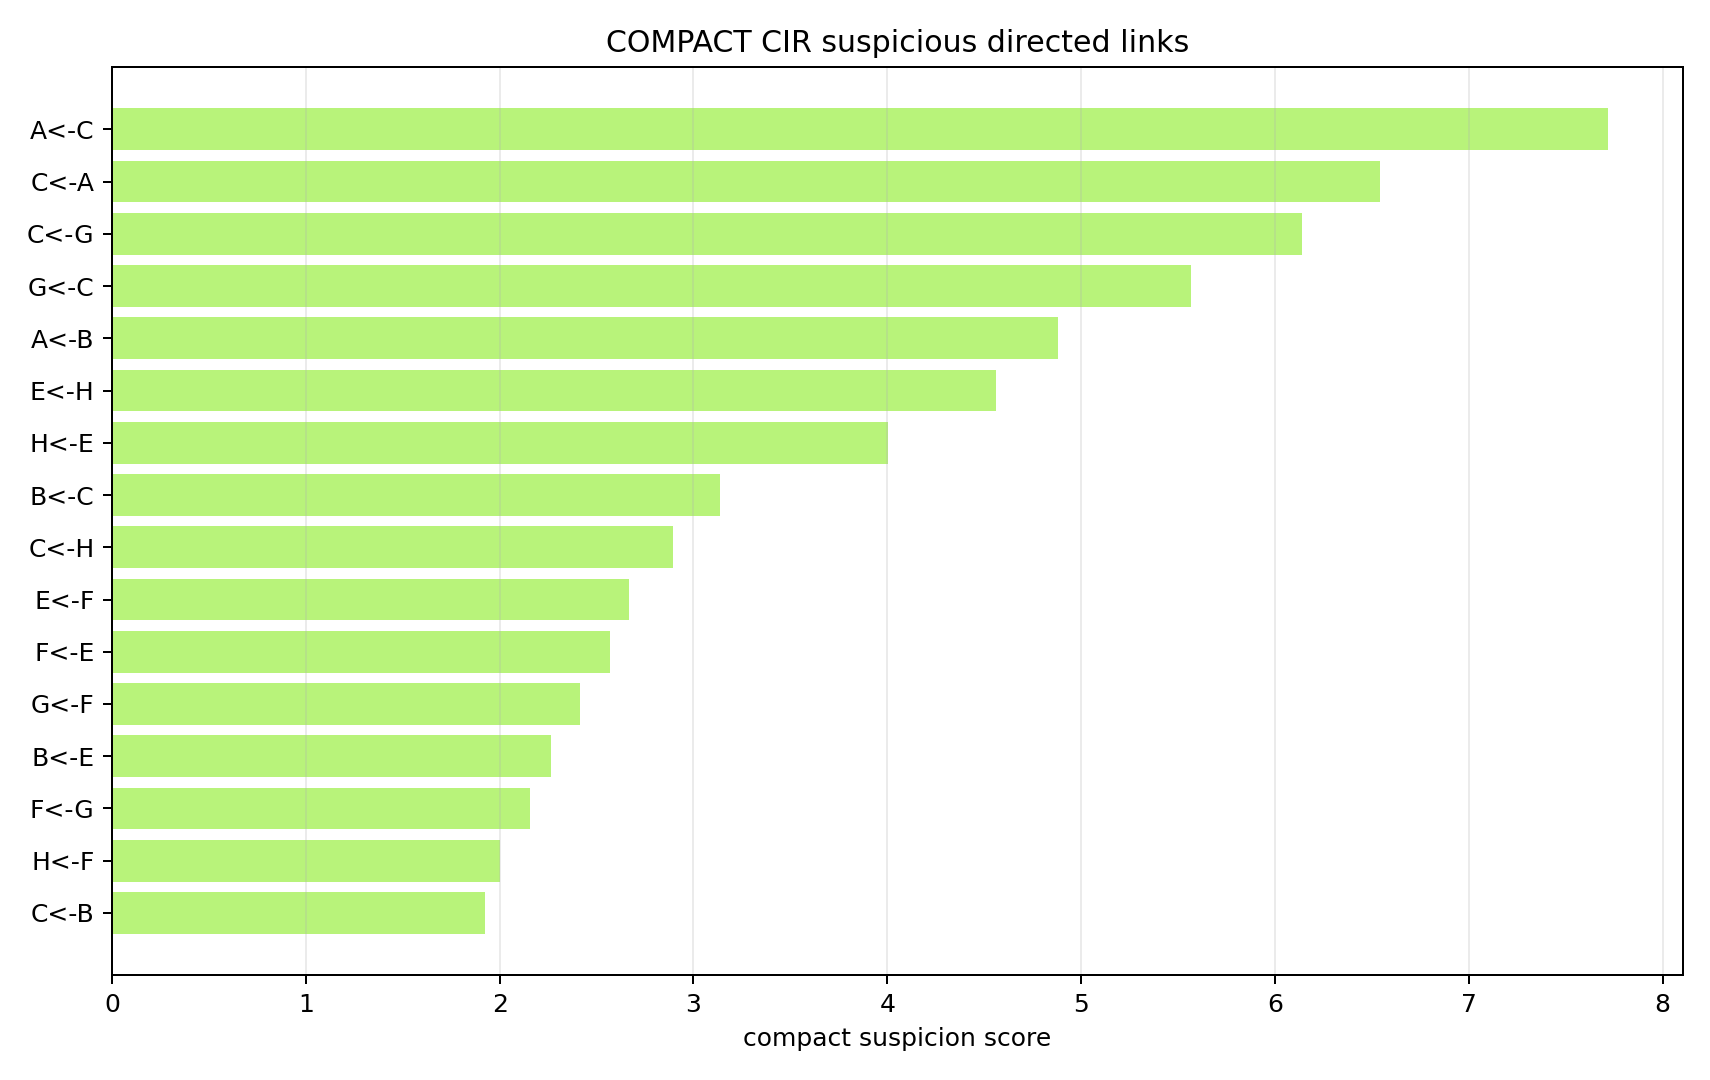
\includegraphics[width=\textwidth]{cir_compact_suspicious_links.png}
\caption{Top suspicious directed links}
\end{subfigure}
\caption{COMPACT CIR 不能重建 full waveform，但可以用 first-path amplitude、peak/fp、noise 和 raw-distance stability 形成 pair-level 质量特征。}
\end{figure}

COMPACT CIR sweep 记录了 952 个 compact ACRX samples，覆盖 56 个 directed links。它无法画出 full accumulator waveform，但可以生成 pair quality features。最高 suspicious directed links 包括 \case{A<-C}、\case{C<-A}、\case{C<-G}、\case{G<-C}、\case{A<-B}、\case{E<-H}、\case{H<-E}。这些结果和 FULL CIR 中的高 tail/弱 SNR links 有部分一致性，说明 compact features 可以作为工程上更轻量的 link-quality proxy。

已有的 CIR-weighted layout smoke test 只证明了 solver 可以消费 CIR-derived pair weights；它尚未证明定位精度已经改善。该 smoke test 中 baseline RMS edges 为 $79.437\mm$，CIR-weighted 为 $82.467\mm$，说明当前权重公式不是最终结果。报告中应明确写成：CIR 目前最有价值的是解释现象和提供未来 weighting/filtering 接口；真正要成为系统结果，还需要把 CIR weight 与静态 tag、RotoArm UWB-Tag、Vicon Motion Capture System truth 做闭环验证。

\section{建议报告结构}

如果最终要写成正式实验报告，建议采用如下结构：
\begin{enumerate}
\item Introduction：说明目标是验证 AutoPos UWB 自部署和 tag localization，不是只优化单一 solver 数字。
\item Dataset and Coordinate Systems：解释 Vicon Motion Capture System、AutoPos layout、tag replay、RotoArm UWB-Tag。
\item AutoPos Anchor Layout：报告 SE(3) 和 Sim(3) layout error。
\item Delay-layout Coupling：用四组对照说明 delay calibration 不能脱离 layout。
\item Static Tag Localization：使用 AutoPos Solver 与 UWB-Tag solver 组合 \case{v4-io/T4} 的 $72.7/171.5/109.8\mm$ 作为主结果。
\item Dynamic RotoArm UWB-Tag Evaluation：报告 $105.8/231.8/141.3\mm$，并解释为什么不是简单时序误差。
\item Robustness and Simulation：放 Monte Carlo keep-k、wall NLOS simulation。
\item CIR Multipath Evidence：用 FULL/COMPACT CIR 展示 clear LOS 下仍存在 tail energy、link-quality difference 和 pair weighting 潜力。
\item Phase 4 UWB+IMU：详细讨论 L2/L16/L20 三类 IMU 的动态融合证据。
\item Limitations：Vicon Motion Capture System 依赖、单场地、CIR weight 尚未闭环验证、IMU 尚未完全实机闭环。
\item Conclusion：重申系统可用性、主要误差机制、下一步路线。
\end{enumerate}

\section{结论}

本次实验最强的科学结论是：AutoPos UWB 自定位在真实场地中已经能够形成可用 anchor geometry，并支持约 $7$--$11$ cm 级的静态 UWB-Tag 定位表现；但 UWB 系统的最终精度不是布局一个变量决定的，而是 layout、delay、solver、动态运动和环境传播共同决定的。AutoPos Solver 与 UWB-Tag solver 组合 \case{v4-io/T4} 应作为静态主结果；RotoArm UWB-Tag 应作为动态挑战展示；Monte Carlo 和 wall NLOS simulation 应作为稳健性与误差来源分析；FULL/COMPACT CIR 应作为 clear LOS 下仍存在 multipath 和 link-quality difference 的物理证据；Phase 4 UWB+IMU 则是当前最明确的动态鲁棒性扩展方向。

\end{document}
